\section{Event Selection}

\begin{frame}{Signal MC Samples}
\begin{columns}
      \begin{column}{0.5\textwidth}
\begin{center}
%\scriptsize
\footnotesize
\begin{tabular}{|c|c|}
\hline
$M_H$ GeV & $\sigma\times$ Br($H \rightarrow ZZ \rightarrow 2l2q$) [pb] \\ \hline
%200  &  0.2566 \\ % \hline
% 210  &  0.2538  \\ % \hline
% 220  &  0.2416  \\ % \hline
 230  &  0.2278  \\ % \hline
 250  &  0.2022 \\ % \hline
 275  &  0.1751  \\ % \hline
 300  &  0.1563  \\ % \hline
 325  &  0.1478  \\ % \hline
 350  &  0.1482  \\         
 375  &  0.1360  \\       
 400  &  0.1111 \\ % \hline
 425  &  0.0914 \\ % \hline
 450  &  0.7311 \\ % \hline
 475  &  0.6000 \\ % \hline
 500  &  0.4719 \\ % \hline
  525  &  0.0380 \\ % \hline
  550  &  0.0305 \\ % \hline
 575  &  0.0250 \\ % \hline
  600  &  0.0201 \\ \hline 
 
\end{tabular}
\end{center}

\end{column}
\begin{column}{0.5\textwidth}
The signal samples, $H \rightarrow ZZ \rightarrow 2l2q$ ($\ell = \mathrm{e}, \mu, \tau$), were simulated with POWHEG then using PYTHIA to do the final parton showering and hadronization.
\\
\vspace{1em}
The cross section times branching fraction for each $m_H$ value is listed in pb. Each sample was generated with 300,000 events.
    \end{column}
  \end{columns}
\end{frame}






\begin{frame}{Background Samples}
%  \begin{itemize}
%  \item
%    Data is Double Electron and Double Muon datasets.
%  \item
%    Background Monte Carlo is primaraly Z+Jets make with the MADGRAPH.
%  \item
%    Other Backgrounds are TT, WW, WZ, ZZ with PYTHIA.
%  \item
%    The signal Monte Carlo samples are POWHEG.
%  \end{itemize}

\begin{center}
Background\\
\footnotesize
\begin{tabular}{|l|l|c|c|}
\hline
Process & generator & $\sigma$ [pb]& luminosity [$\invfb$] \\
\hline 
$Z$+jets (inclusive)       & madgraph & 3503.71 & 8.7 \\
 & & & \\
$Z$+1 jet (exclusive)      & madgraph & 660.6 & 36.4\\
$Z$+2 jet (exclusive)     & madgraph & 215.1 & 101.6 \\
$Z$+3 jet (exclusive)     & madgraph & 65.79 & 167.4 \\
$Z$+4 jet (exclusive)     & madgraph & 27.59 & 232.1 \\
 & & & \\
$\Pqt \Paqt$ & powheg-pythia6 & 23.38 & 461 \\
$ZZ$ & pythia6 & 17.654 & 549 \\
$WZ$ & pythia6 & 22.88 & 424 \\
$WW$ & pythia6 & 57.1097 & 168 \\
\hline
\end{tabular}
\end{center}

\end{frame}




\begin{frame}{Datasets (19.6 $fb^{-1}$)}
Double Electron and Double Muon datasets from a total of 19.6 $fb^{-1}$ collected data in 2012 at $\sqrt{s}$ = 8 TeV.\\
\vspace{1em}
\scriptsize
\begin{tabular}{|l|l|r|}
\hline
Channel & Dataset & Luminosity [pb$^{-1}$] \\
\hline
$2\mu2q$ & /DoubleMu/Run2012A-13Jul2012-v1/AOD & 808\\
         & /DoubleMu/Run2012A-recover-06Aug2012-v1/AOD & 82\\
         & /DoubleMu/Run2012B-13Jul2012-v4/AOD & 4429 \\
         & /DoubleMu/Run2012C-24Aug2012-v1/AOD & 495 \\
         & /DoubleMu/Run2012C-EcalRecover\_11Dec2012-v1/AOD & 134\\
         & /DoubleMu/Run2012C-PromptReco-v2/AOD & 6394\\
         & /DoubleMu/Run2012D-PromptReco-v1/AOD & 7274\\
\hline 
$2e2q$   & /DoubleElectron/Run2012A-13Jul2012-v1/AOD & 808\\
         & /DoubleElectron/Run2012A-recover-06Aug2012-v1/AOD & 82\\
         & /DoubleElectron/Run2012B-13Jul2012-v4/AOD & 4429\\
         & /DoubleElectron/Run2012C-24Aug2012-v1/AOD & 495\\
         & /DoubleElectron/Run2012C-EcalRecover\_11Dec2012-v1/AOD & 134\\
         & /DoubleElectron/Run2012C-PromptReco-v2/AOD & 6394\\
         & /DoubleElectron/Run2012D-PromptReco-v1/AOD & 7274\\
%\hline 
%$e\mu qq$& /MuEG/Run2012A-13Jul2012-v1/AOD & 808\\
%         & /MuEG/Run2012A-recover-06Aug2012-v1/AOD & 82\\
%         & /MuEG/Run2012B-13Jul2012-v4/AOD & 4429\\
%         & /MuEG/Run2012C-24Aug2012-v1/AOD & 495\\
%         & /MuEG/Run2012C-EcalRecover\_11Dec2012-v1/AOD & 134\\
%         & /MuEG/Run2012C-PromptReco-v2/AOD & 6394\\
%         & /MuEG/Run2012D-PromptReco-v1/AOD & 7274\\
\hline
\end{tabular}

\end{frame}



\begin{frame}{Particle Flow}
The particle flow algorithm attempts to reconstruct all stable final state particles using all of the CMS sub-detectors.

\begin{columns}[T]
  \begin{column}{0.6\textwidth}
\footnotesize
%\scriptsize
    \begin{itemize}
    \item
      1. Create electrons for all tracks linked to a single ECAL cluster that pass the electron ID.
    \end{itemize}
  \end{column}
  \begin{column}{0.40\textwidth}
    \includegraphics[width=0.99\textwidth]{images/pf1.pdf}
  \end{column}
\end{columns}
\end{frame}



\begin{frame}{Particle Flow}
The particle flow algorithm attempts to reconstruct all stable final state particles using all of the CMS sub-detectors.

\begin{columns}[T]
  \begin{column}{0.6\textwidth}
\footnotesize
%\scriptsize
    \begin{itemize}
    \item
      1. Create electrons for all tracks linked to a single ECAL cluster that pass the electron ID.
    \item
      2. If the tracks fail the electron ID create a charged hadron, unless there are hits in the muon chambers, then create a muon.
    \end{itemize}
  \end{column}
  \begin{column}{0.40\textwidth}
    \includegraphics[width=0.99\textwidth]{images/pf2.pdf}
  \end{column}
\end{columns}
\end{frame}


\begin{frame}{Particle Flow}
The particle flow algorithm attempts to reconstruct all stable final state particles using all of the CMS sub-detectors.

\begin{columns}[T]
  \begin{column}{0.6\textwidth}
\footnotesize
%\scriptsize
    \begin{itemize}
    \item
      1. Create electrons for all tracks linked to a single ECAL cluster that pass the electron ID.
    \item
      2. If the tracks fail the electron ID create a charged hadron, unless there are hits in the muon chambers, then create a muon.
    \item
      3. For each HCAL cluster get all the linked tracks and ECAL clusters. Create a charged hadron for each track. If the energy in the HCAL is greater than the energy in the tracks, create photons or neutral hadrons equal to the missing energy.
    \end{itemize}
  \end{column}
  \begin{column}{0.40\textwidth}
    \includegraphics[width=0.99\textwidth]{images/pf3.pdf}
  \end{column}
\end{columns}
\end{frame}

\begin{frame}{Particle Flow}
The particle flow algorithm attempts to reconstruct all stable final state particles using all of the CMS sub-detectors.

\begin{columns}[T]
  \begin{column}{0.6\textwidth}
\footnotesize
%\scriptsize
    \begin{itemize}
    \item
      1. Create electrons for all tracks linked to a single ECAL cluster that pass the electron ID.
    \item
      2. If the tracks fail the electron ID create a charged hadron, unless there are hits in the muon chambers, then create a muon.
    \item
      3. For each HCAL cluster get all the linked tracks and ECAL clusters. Create a charged hadron for each track. If the energy in the HCAL is greater than the energy in the tracks, create photons or neutral hadrons equal to the missing energy.
    \item
      4. For the remaining ECAL (HCAL) clusters that are not linked to tracks create a photon (neutral hadron).
    \end{itemize}
  \end{column}
  \begin{column}{0.40\textwidth}
    \includegraphics[width=0.99\textwidth]{images/pf4.pdf}
  \end{column}
\end{columns}
\end{frame}















\begin{frame}{PileUp and Isolation}
\begin{columns}
\begin{column}{0.5\textwidth}
\begin{center}
$\beta = \dfrac{\sum_{P_T\ CJP\ from\ Vertex}}{\sum_{P_T\ all\ CJP}}$\\
\footnotesize
 where CJP is charged jet particles.
\includegraphics[width=0.89\textwidth]{images/beta.png}\\
Jets originating from pile-up interactions are removed by cutting on $\beta$ > 0.2.
\end{center}
\end{column}
\begin{column}{0.5\textwidth}
\begin{center}
{\footnotesize We also require that our objects are isolated by cutting on a cone around the primary vertex with radius:}\\
$\Delta R = \sqrt{\Delta \phi^2 + \Delta \eta^2} > 0.5$
\includegraphics[width=0.99\textwidth]{images/JetConeAll-1024x778.png}\\
{\fontsize{.1cm}{.001em}\selectfont Source: \url{http://www.quantumdiaries.org/2011/06/01/anatomy-of-a-jet-in-cms/}}
%∆R = ∆φ2 + ∆η 2 > 0.5
\end{center}
\end{column}
\end{columns}
\end{frame}

\begin{frame}{Analysis workflow}
  \begin{center}
  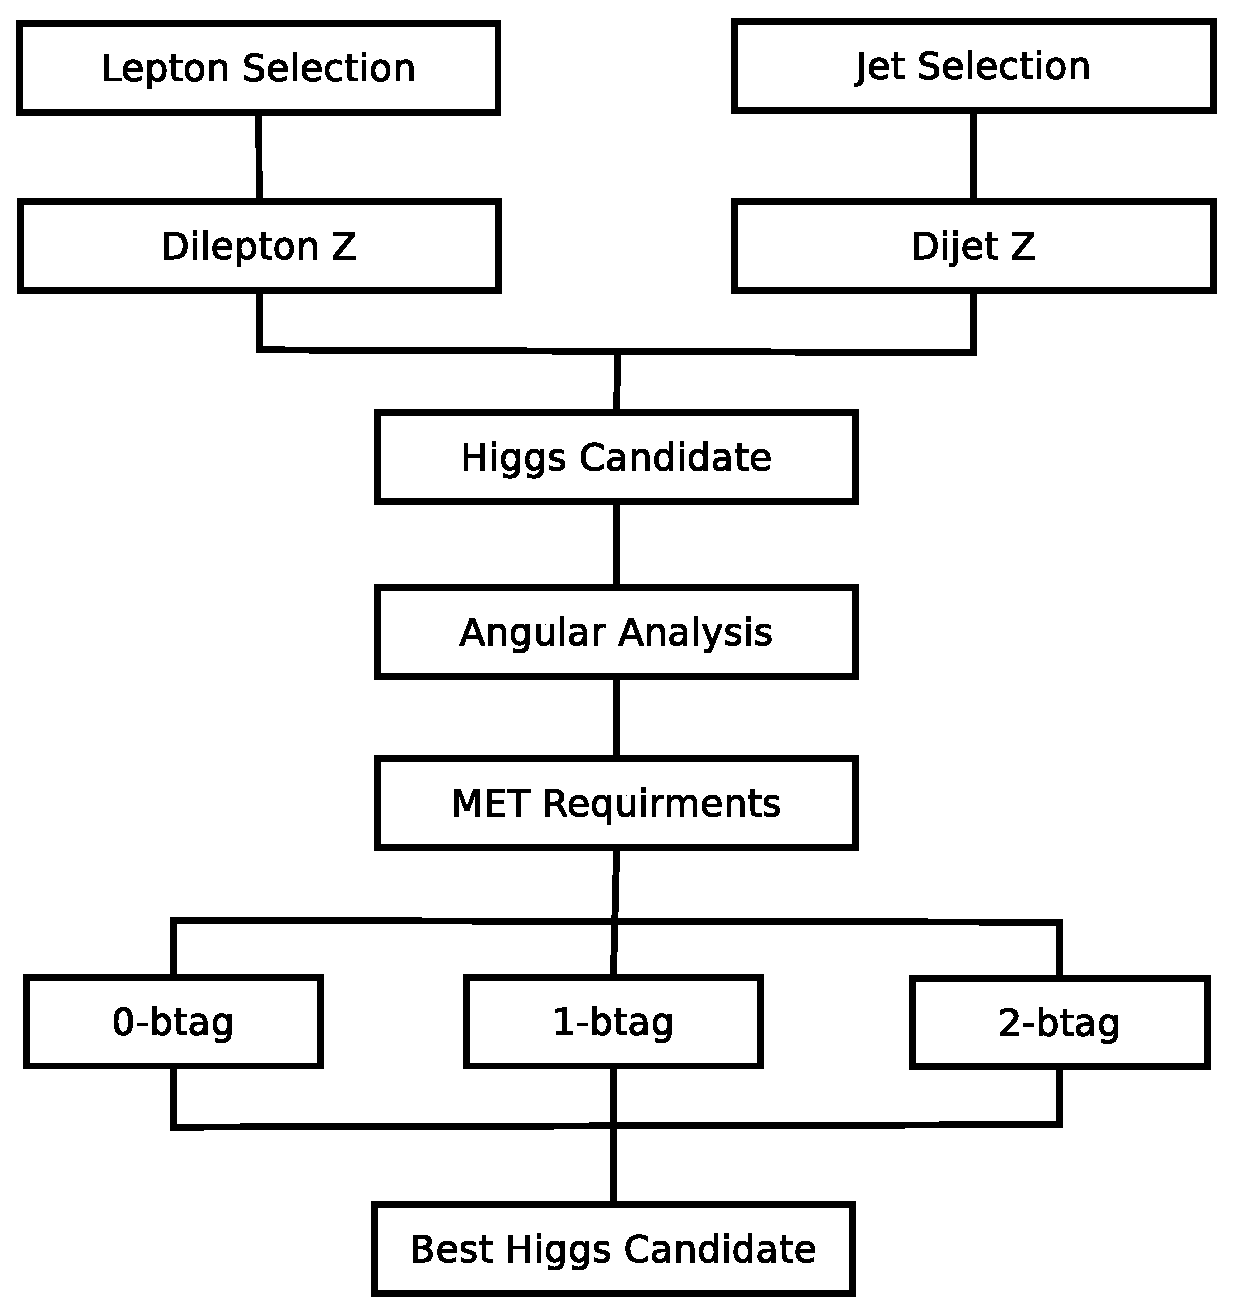
\includegraphics[width=0.6\textwidth]{images/analysis_strategy.eps}
  \end{center}
\end{frame}

\begin{frame}{Physics Objects and Preselection}
\begin{columns}
\begin{column}{0.6\textwidth}
   \footnotesize

 {\bf Triggers}\\
  \begin{itemize}
        \item
          HLT\_Ele17\_CaloIdT\_TrkIdVL\_CaloIsoVL\_\\
          TrkIsoVL\_Ele8\_CaloIdT\_TrkIdVL\_CaloIsoVL\_\\
          TrkIsoVL
        \item
          HLT\_Mu17\_Mu8
\end{itemize}

\vspace{2em}
We are using the recomendations from the CMS physics object groups for lepton identification and isolation.  These values can be seen in the backup slides.

\vspace{1em}

After we have the objects, we apply additional preselection cuts to the leptons.
%  We keep each combination that satisfy the criteria as a candidate even if there are multiple per event.

 % 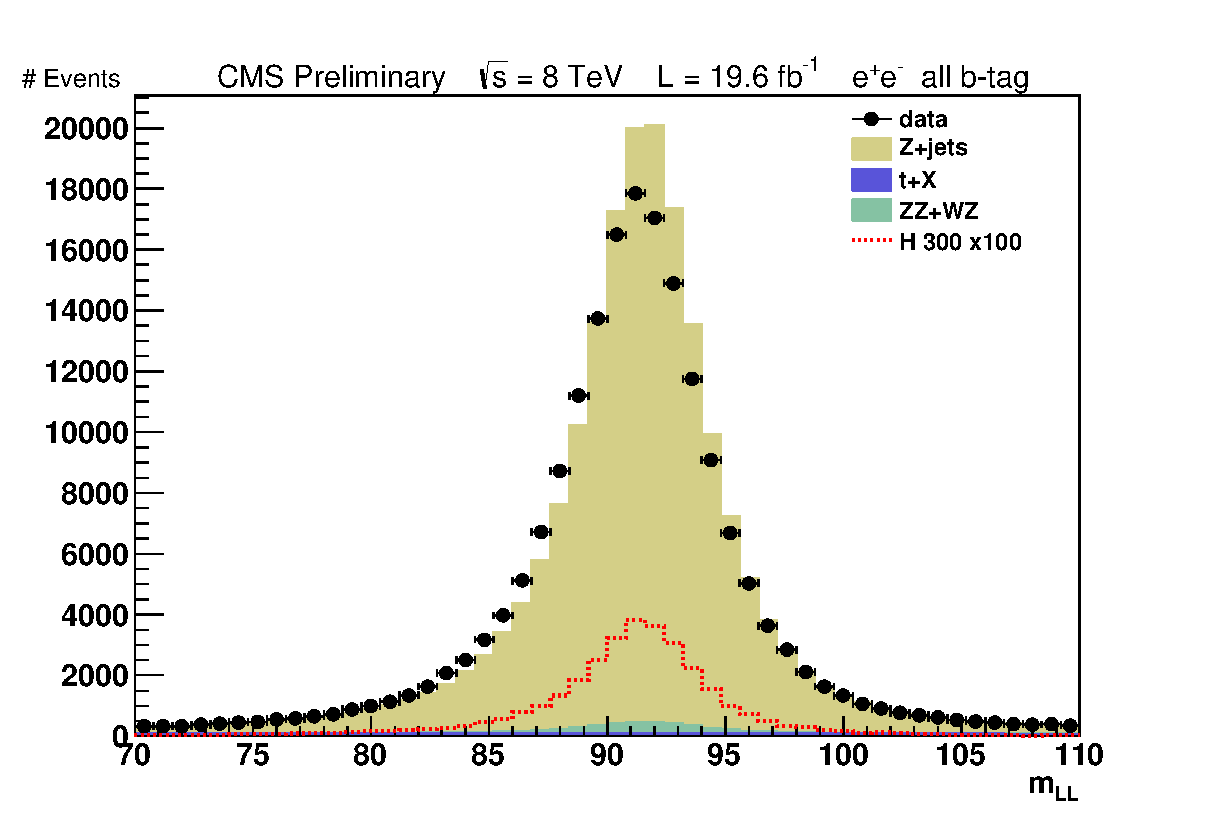
\includegraphics[width=0.8\textwidth]{images/preselection/el/mLL.eps}\\
 % 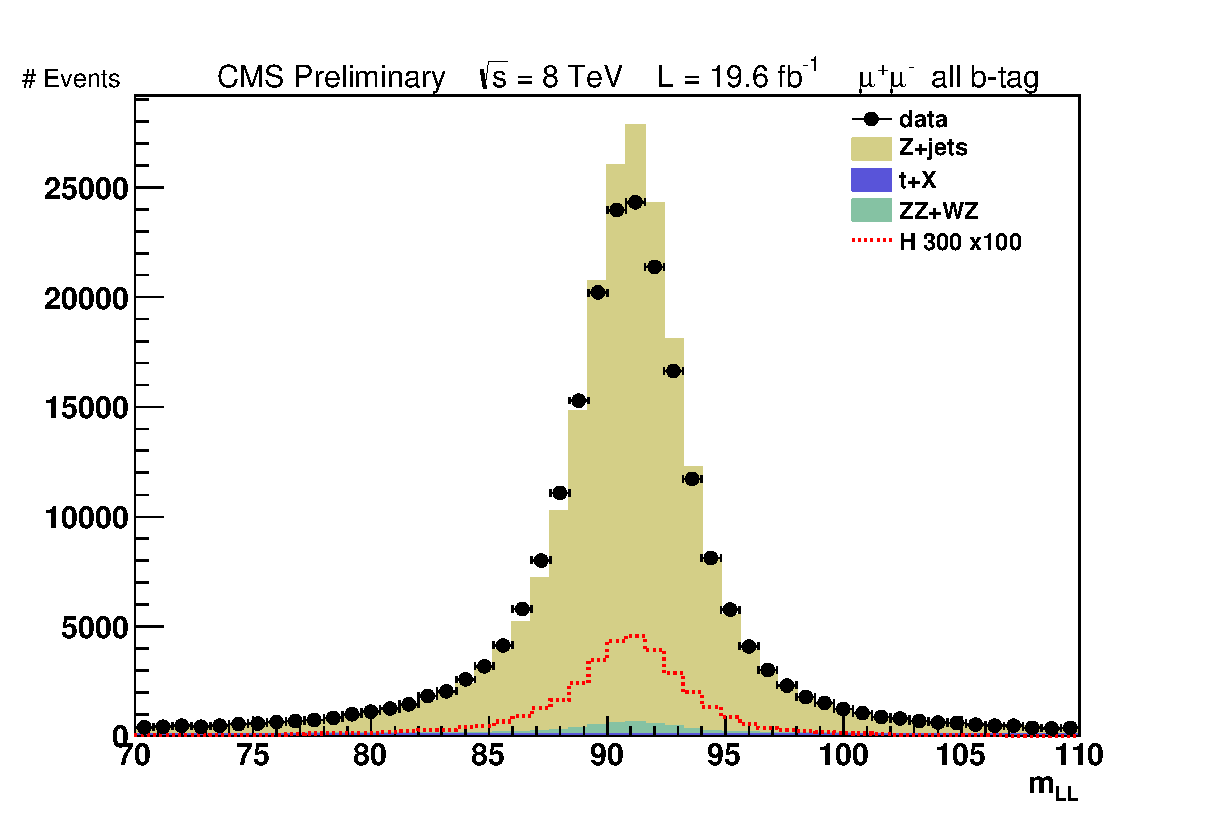
\includegraphics[width=0.8\textwidth]{images/preselection/mu/mLL.eps}
\end{column}


      \begin{column}{0.4\textwidth}
        \footnotesize
        \scriptsize
  %        {\bf Leptons}\\
  {\bf Electrons}\\
  Physics Object
  \begin{itemize}
    \footnotesize
  \item
    Identification and Isolation
    \end{itemize}
  Preselection
  \begin{itemize}
  \item
    $p_{T}$ > 40/20 GeV
  \item
    $|\eta|$ < 2.5
  \end{itemize}

  {\bf Muons}\\
  Physics Object
  \begin{itemize}
    \footnotesize
    %\scriptsize
  \item
    Identification and Isolation
    \end{itemize}
  Preselection
  \begin{itemize}
  \item
    $p_{T}$ > 40/20 GeV
  \item
    $|\eta|$ < 2.4
  \end{itemize}
 {\bf Jets}\\
        Physics Object
        \begin{itemize}
        \item
          Identification and Isolation
        \end{itemize}
        
        Preselection
        \begin{itemize}
        \item
          p$_{T}$ > 30 GeV
        \item
          $|\eta|$ < 2.4
        \end{itemize}


  \end{column}
      
\end{columns}
\end{frame}


\begin{frame}{Mass Cut around Z$_{jj}$ Peak}
\begin{center}
Our main background is Z+jets where the Z decays into leptons.  For the signal the di-jet mass peak should be at the nominal Z boson mass of 91 GeV.  We can cut on either side of this peak to reject a large amount of the Z+jets background. We optimized these cuts to maximize $\dfrac{S}{\sqrt{S+B}}$.
\\
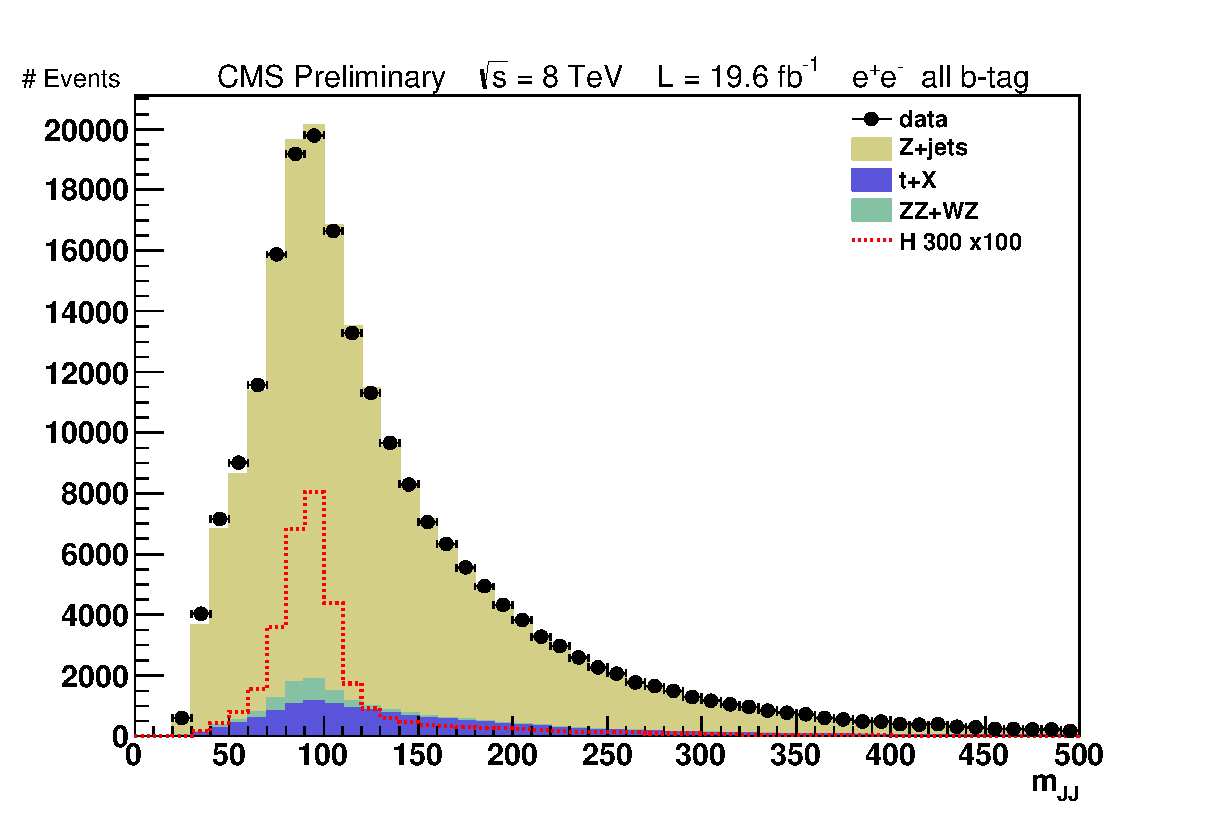
\includegraphics[width=0.5\textwidth]{images/preselection/el/mJJ.eps}
\includegraphics[width=0.5\textwidth]{images/test_zjj_s_sb_zero.eps}
%\includegraphics[width=0.33\textwidth]{images/zjj_s_sb_one.eps}
%\includegraphics[width=0.33\textwidth]{images/zjj_s_sb_two.eps}
\end{center}
\end{frame}

\begin{frame}{Signal and Sideband Regions}
  \begin{columns}
    \begin{column}{0.6\textwidth}
\footnotesize
\scriptsize
Optimal cuts around the Z$_{ll}$ mass peak were also calculated. A side band region is defined in the Z$_{jj}$ mass distribution.  This side band region is used to get the Z+jets background from data.
\\
\footnotesize
\vspace{1em}
      Signal:
      \begin{itemize}
      \item
        76 < m$_{ll}$ < 106 GeV
      \item
        71 < m$_{jj}$ < 111 GeV
      \end{itemize}
      Sideband:
      \begin{itemize}
      \item
        76 < m$_{ll}$ < 106 GeV
      \item
        60 < m$_{jj}$ < 71 GeV\\
        111 < m$_{jj}$ < 130 GeV
      \end{itemize}
\vspace{2em}
\scriptsize
The muon distributions look similar and can be seen in the backup slides.
    \end{column}
    \begin{column}{0.4\textwidth}
      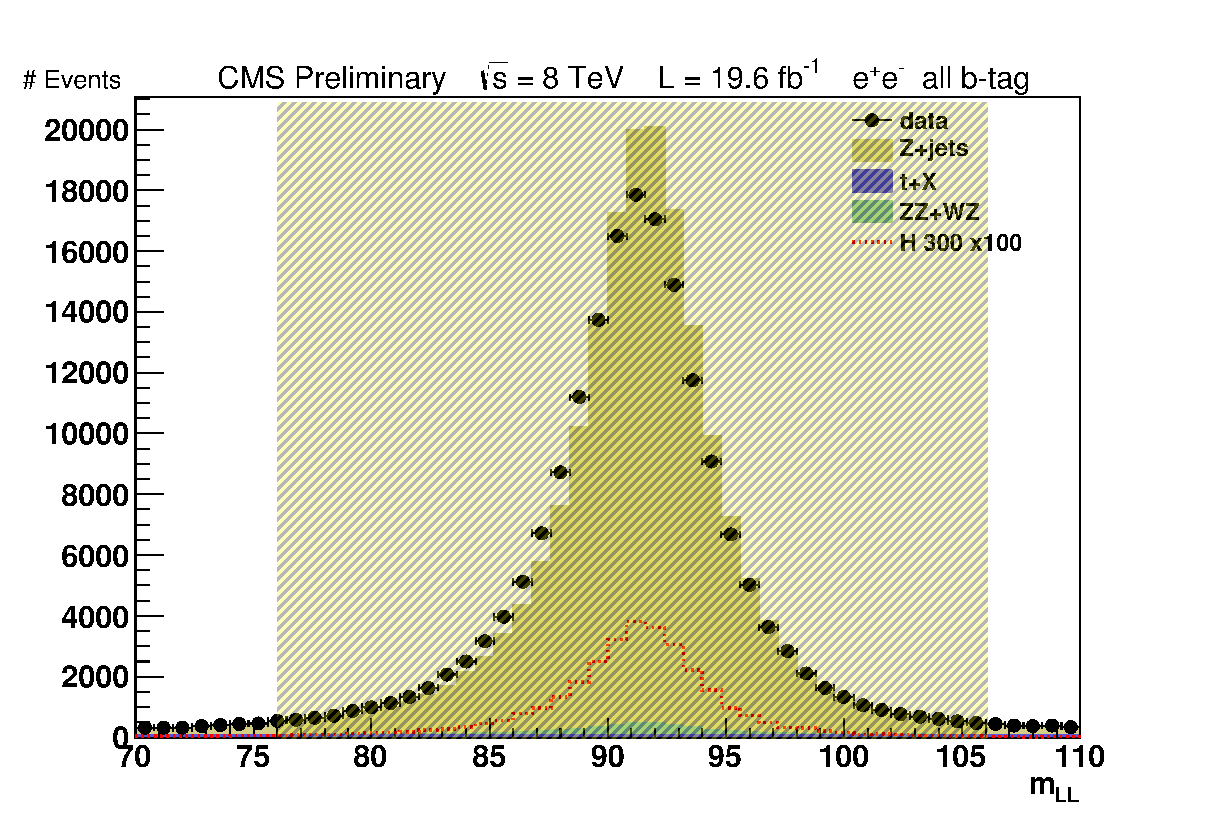
\includegraphics[width=0.99\textwidth]{images/mLL_signal_sideband.eps}\\
      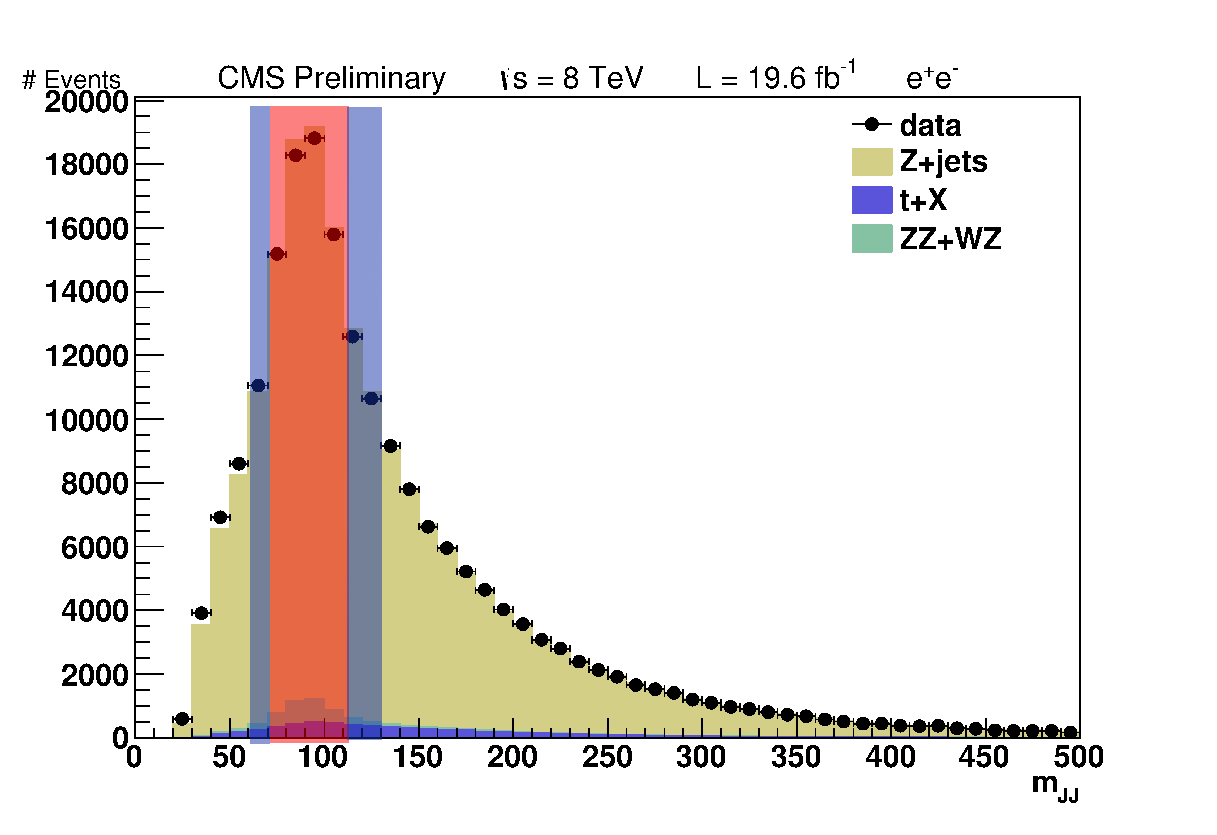
\includegraphics[width=0.99\textwidth]{images/mJJ_signal_sideband.eps}
    \end{column}
  \end{columns}
\begin{center}
\footnotesize
 At this point we keep each combination that satisfy the previous criteria as a Higgs candidate.  There can be multiple Higgs candidates per event at this stage.
%  {\bf Study Regions}
%  \begin{itemize}
%  \item 
%   Signal Region is 76 < m$_{ll}$ < 106 GeV and 71 < m$_{jj}$ < 111 GeV
%  \item 
%    Also we are looking at the sidebands region, defined as 60< m$_{jj}$ <71 GeV || 111< m$_{jj}$ <130 GeV (i.e. outside signal window 75< mjj < 105 GeV).
%  \end{itemize}
 % 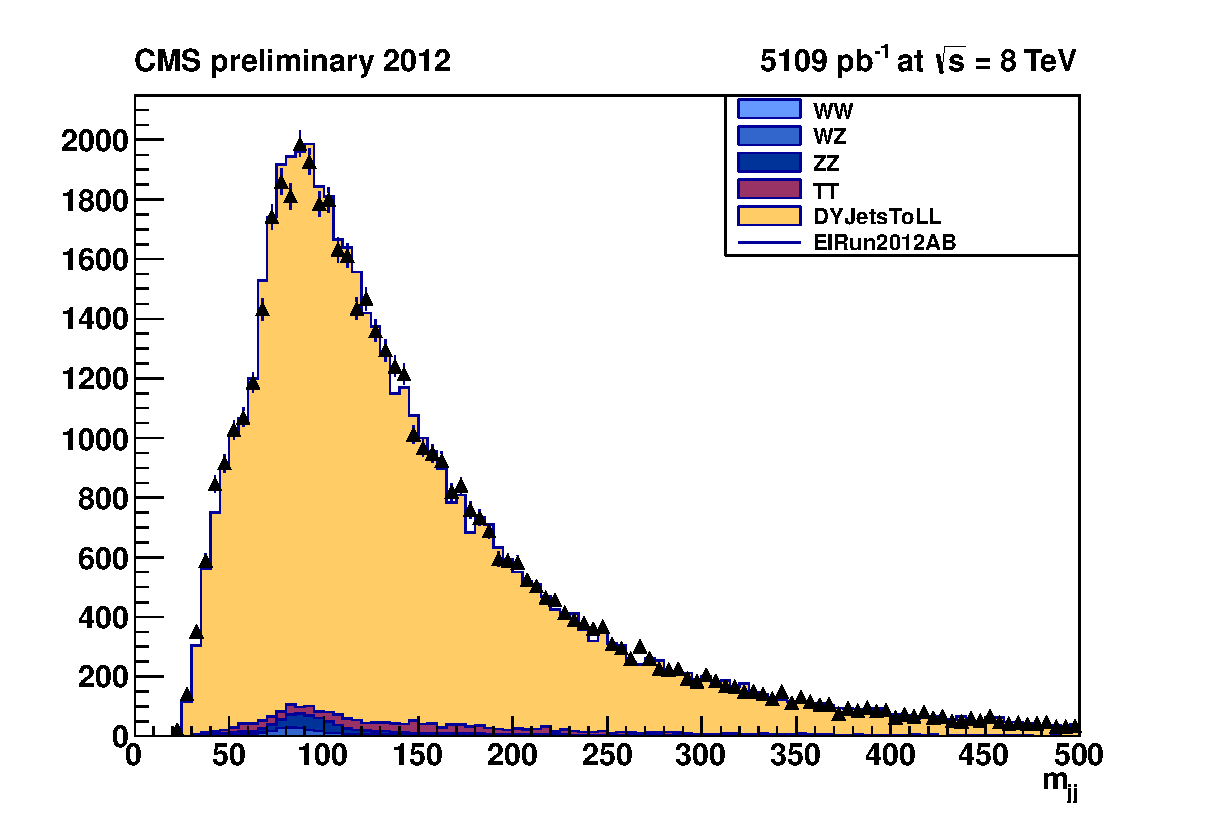
\includegraphics[width=0.5\textwidth]{images/zjjmass_ElRun2012.eps}
 % \includegraphics[width=0.5\textwidth]{images/zjjmass_MuRun2012.eps}
%  \begin{center}
%    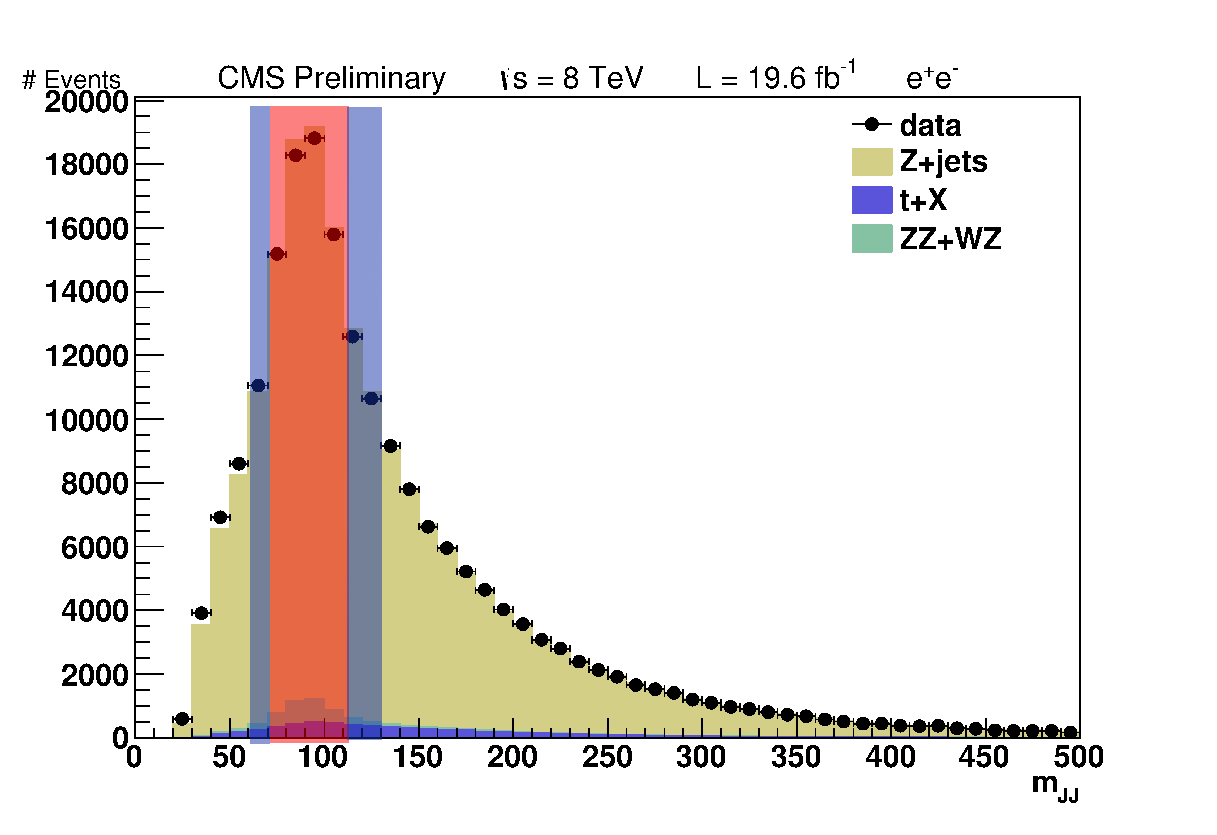
\includegraphics[width=0.6\textwidth]{images/mJJ_signal_sideband.eps}
  \end{center}
\end{frame}

%\begin{frame}{Jets}
%      \begin{itemize}
%      \item
%        AK5PF, L1FastJet+L2+L3  %no MVA ID applied
%      \item
%        p$_{T}$ > 30 GeV
%      \item
%        $|\eta|$ < 2.4
%      \end{itemize}
%  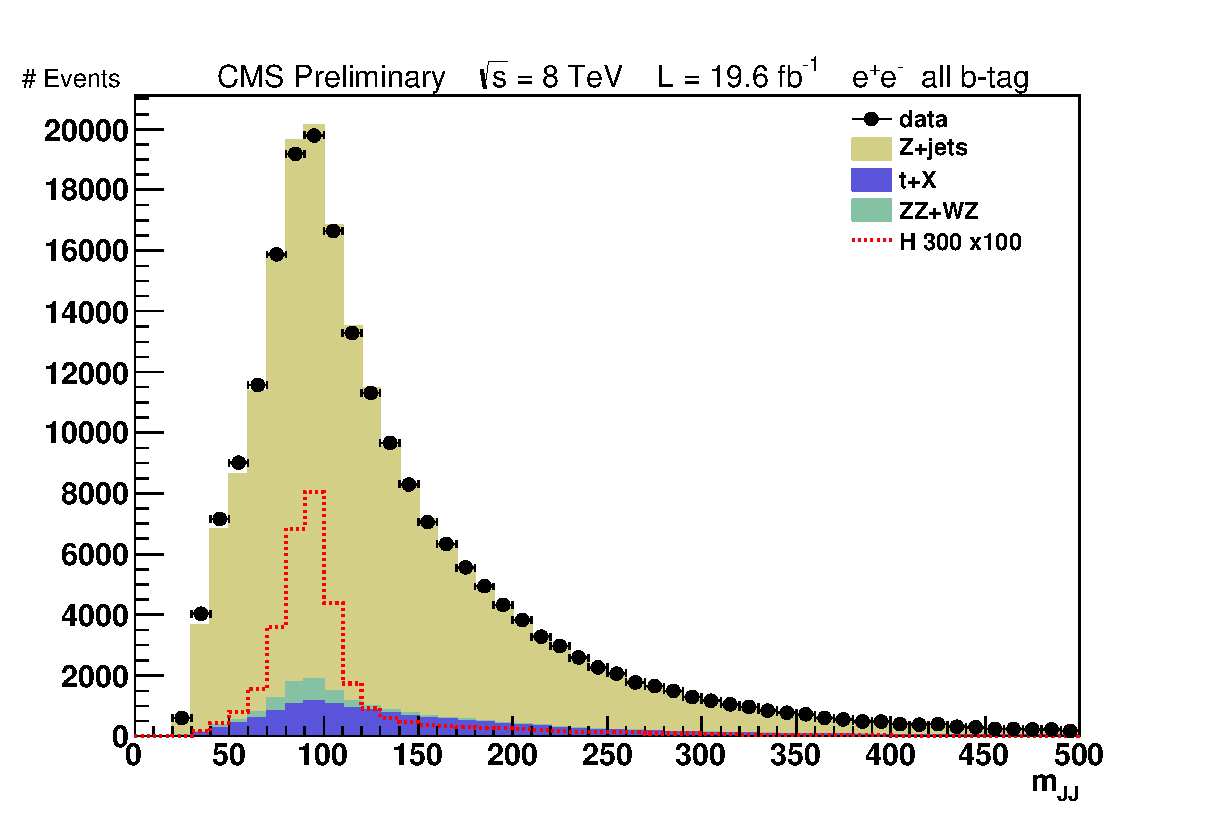
\includegraphics[width=0.5\textwidth]{images/preselection/el/mJJ.eps}
%  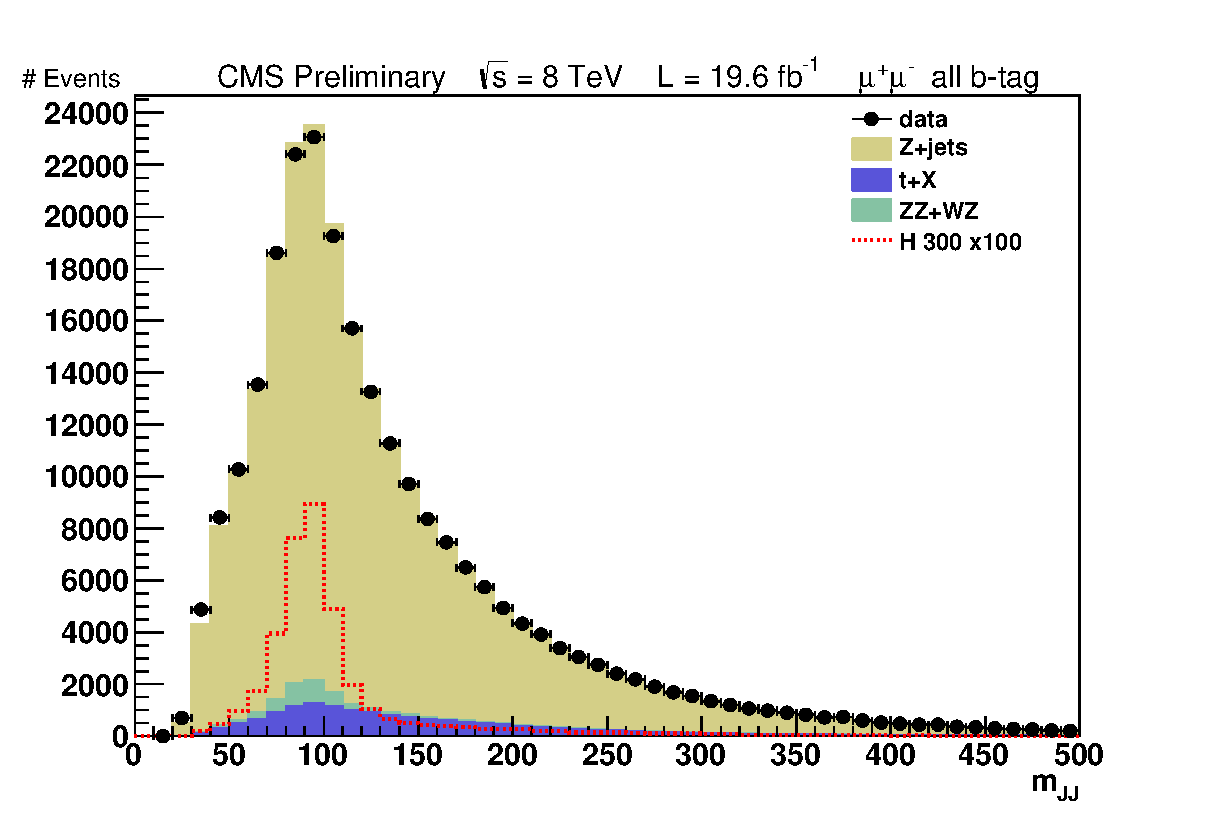
\includegraphics[width=0.5\textwidth]{images/preselection/mu/mJJ.eps}
%\end{frame}

\begin{frame}{Helicity and Production Angles}
\begin{center}
Final state kinematics completely determined by 5 angles.
\includegraphics[width=0.6\textwidth]{images/plots/angles-HZZ2l2q}
\\
$ cos(\theta^*), cos(\theta_1), cos(\theta_2), \Phi, \Phi_1$
\end{center}
\end{frame}


\begin{frame}{Electron Helicity and Production Angles}
\begin{center}
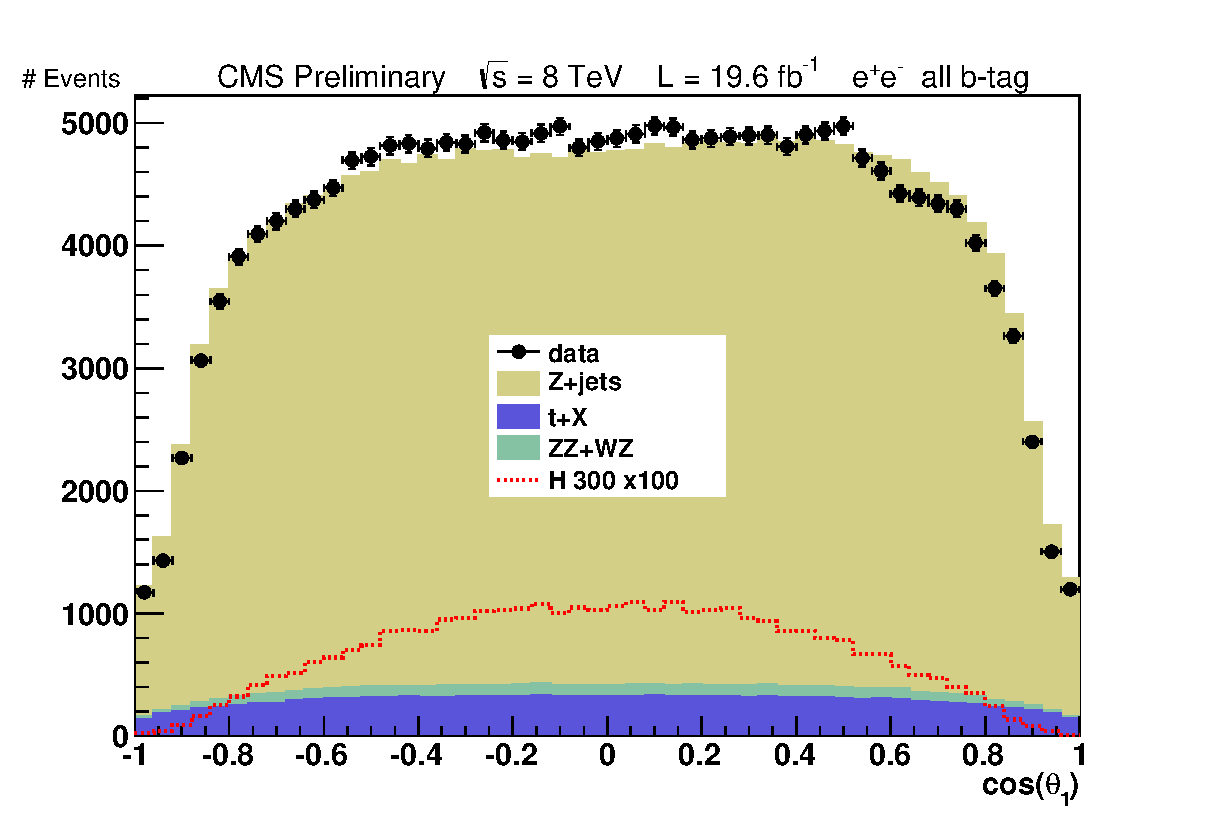
\includegraphics[width=0.33\textwidth]{images/preselection/el/costheta1.eps}
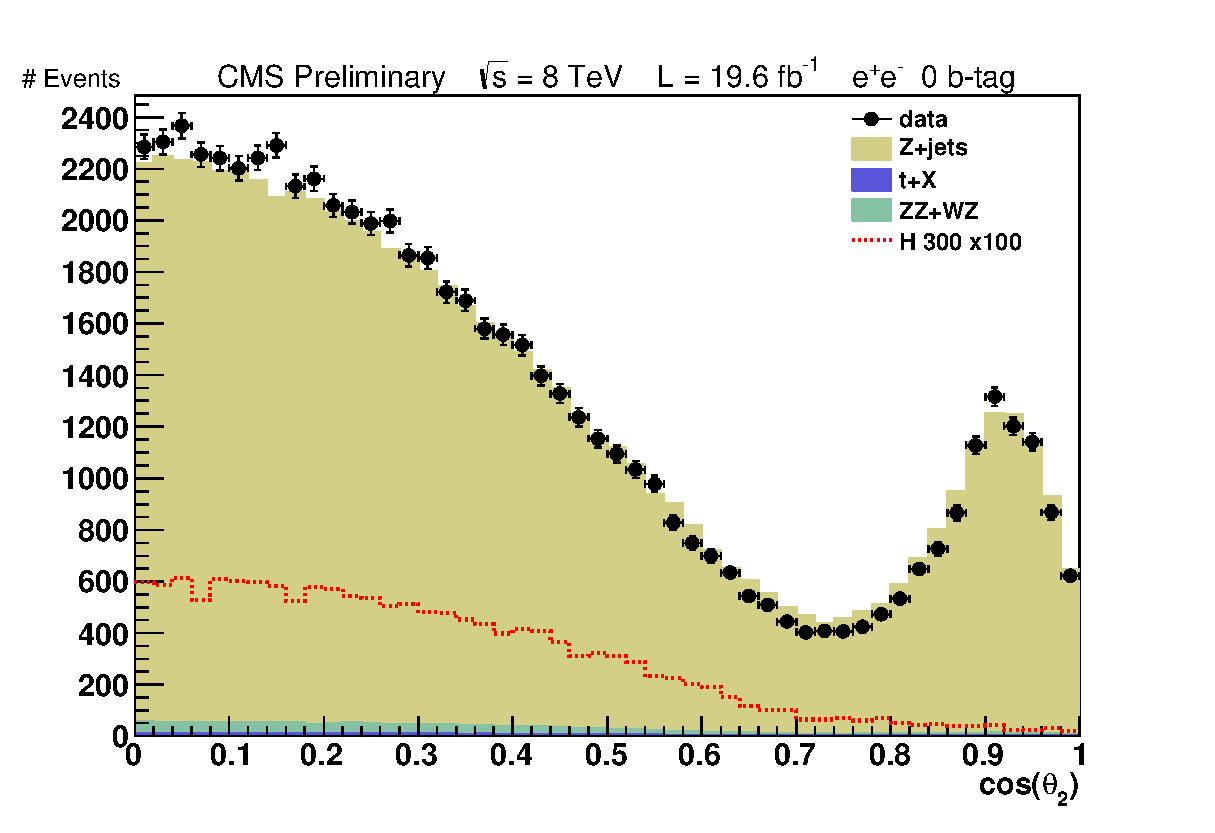
\includegraphics[width=0.33\textwidth]{images/preselection/el/costheta2.eps}
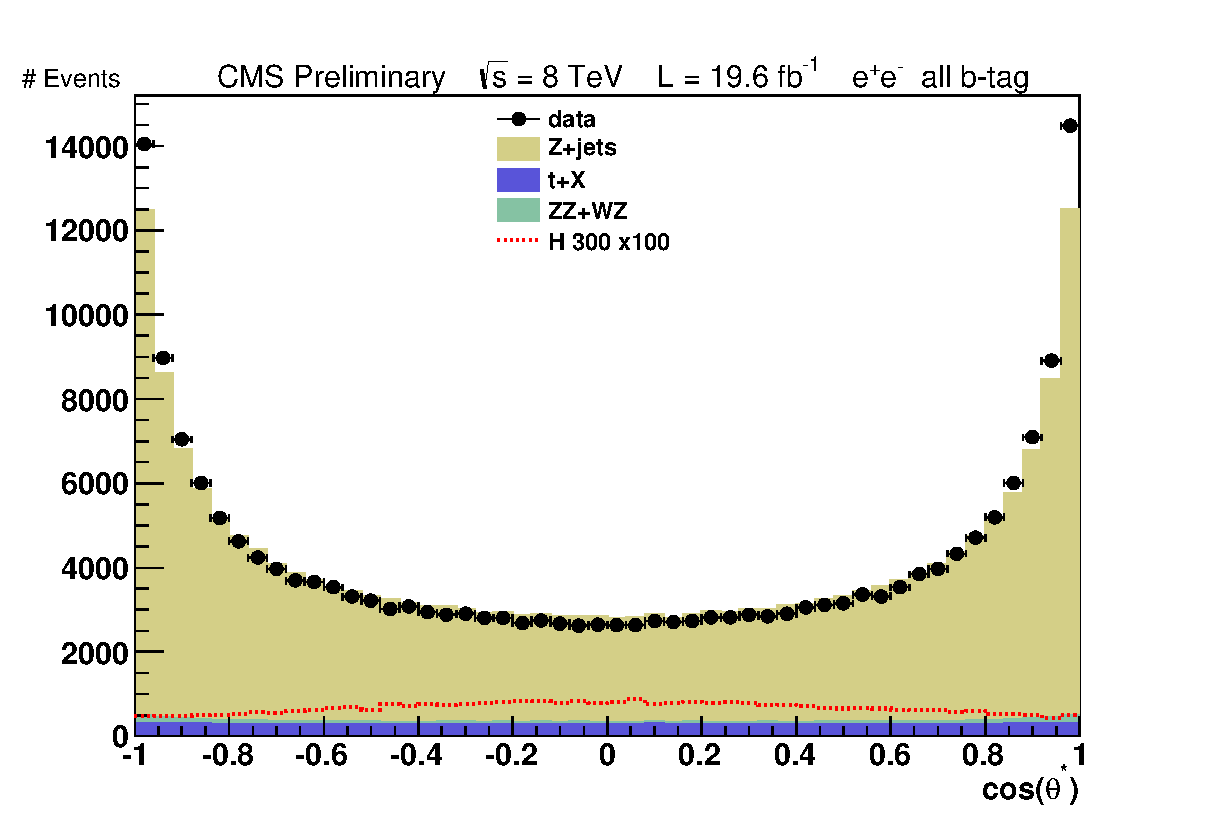
\includegraphics[width=0.33\textwidth]{images/preselection/el/costhetast.eps}
\\
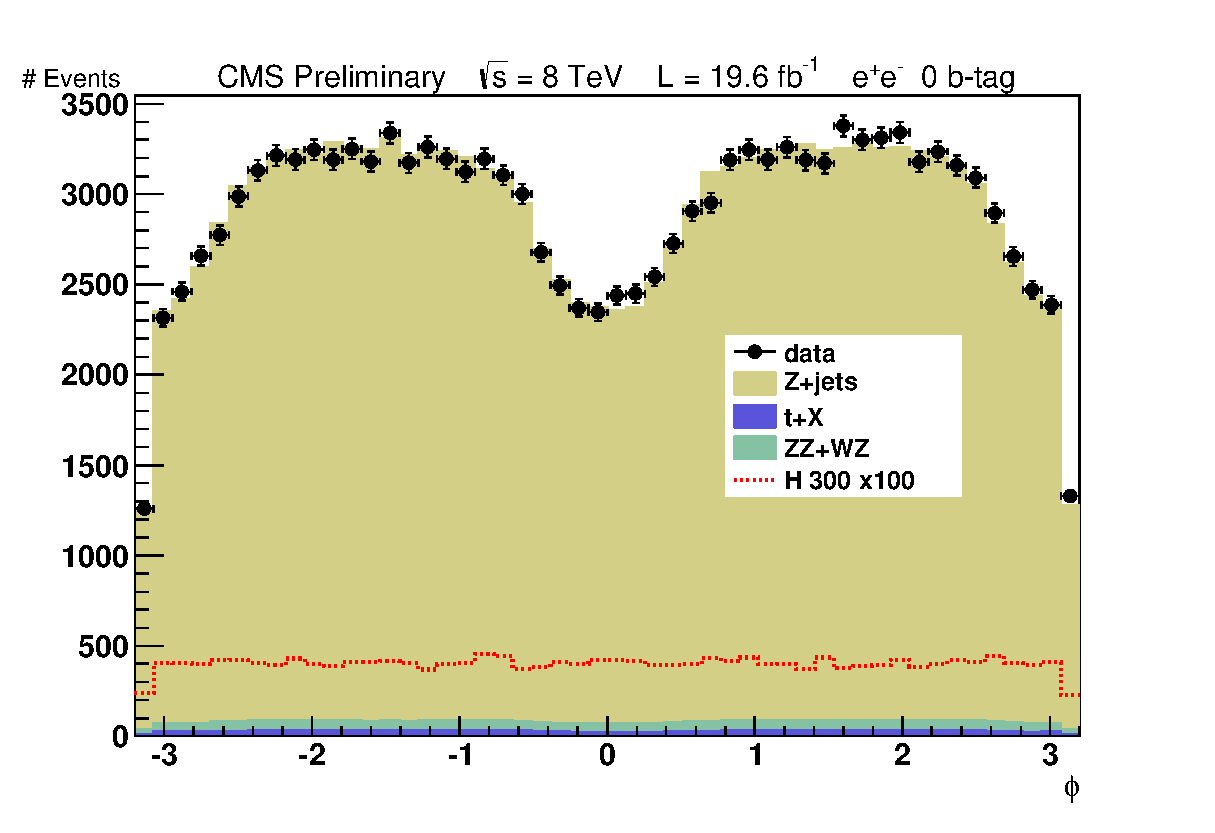
\includegraphics[width=0.33\textwidth]{images/preselection/el/phi.eps}
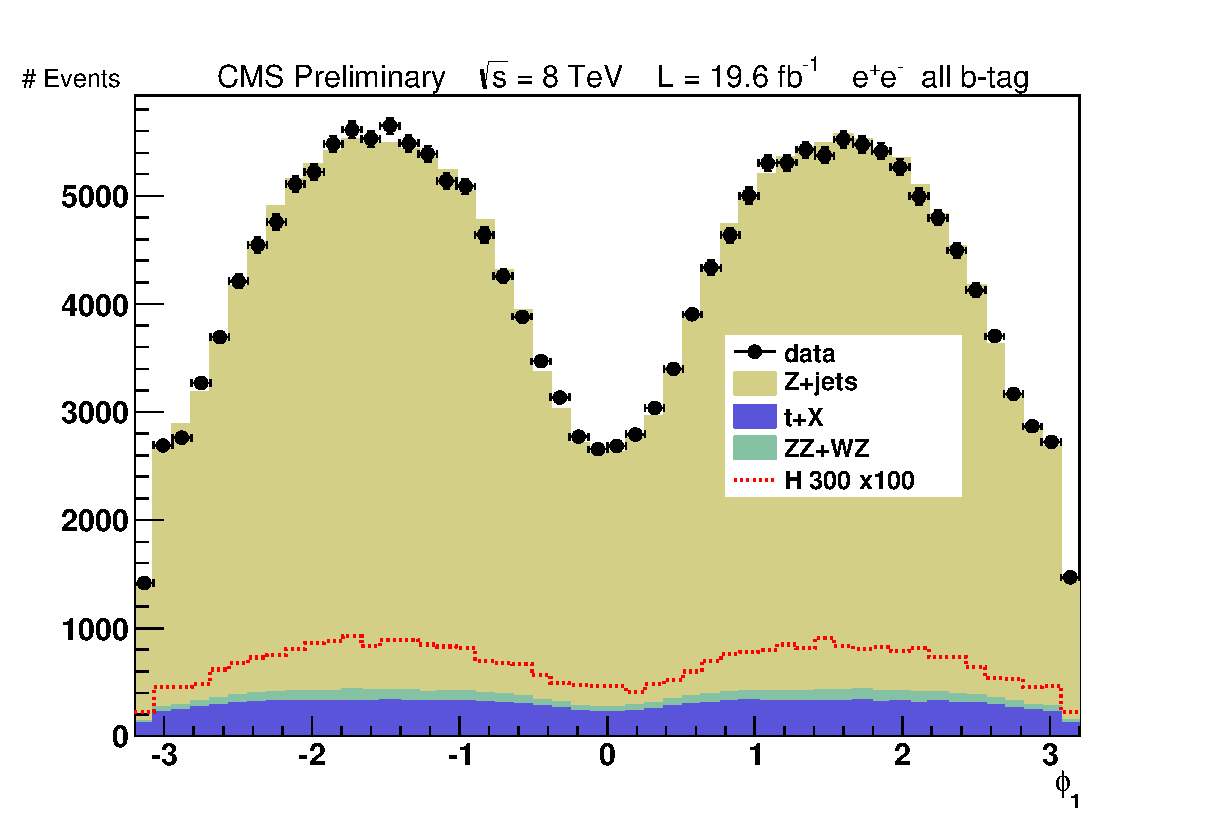
\includegraphics[width=0.33\textwidth]{images/preselection/el/phi1.eps}
%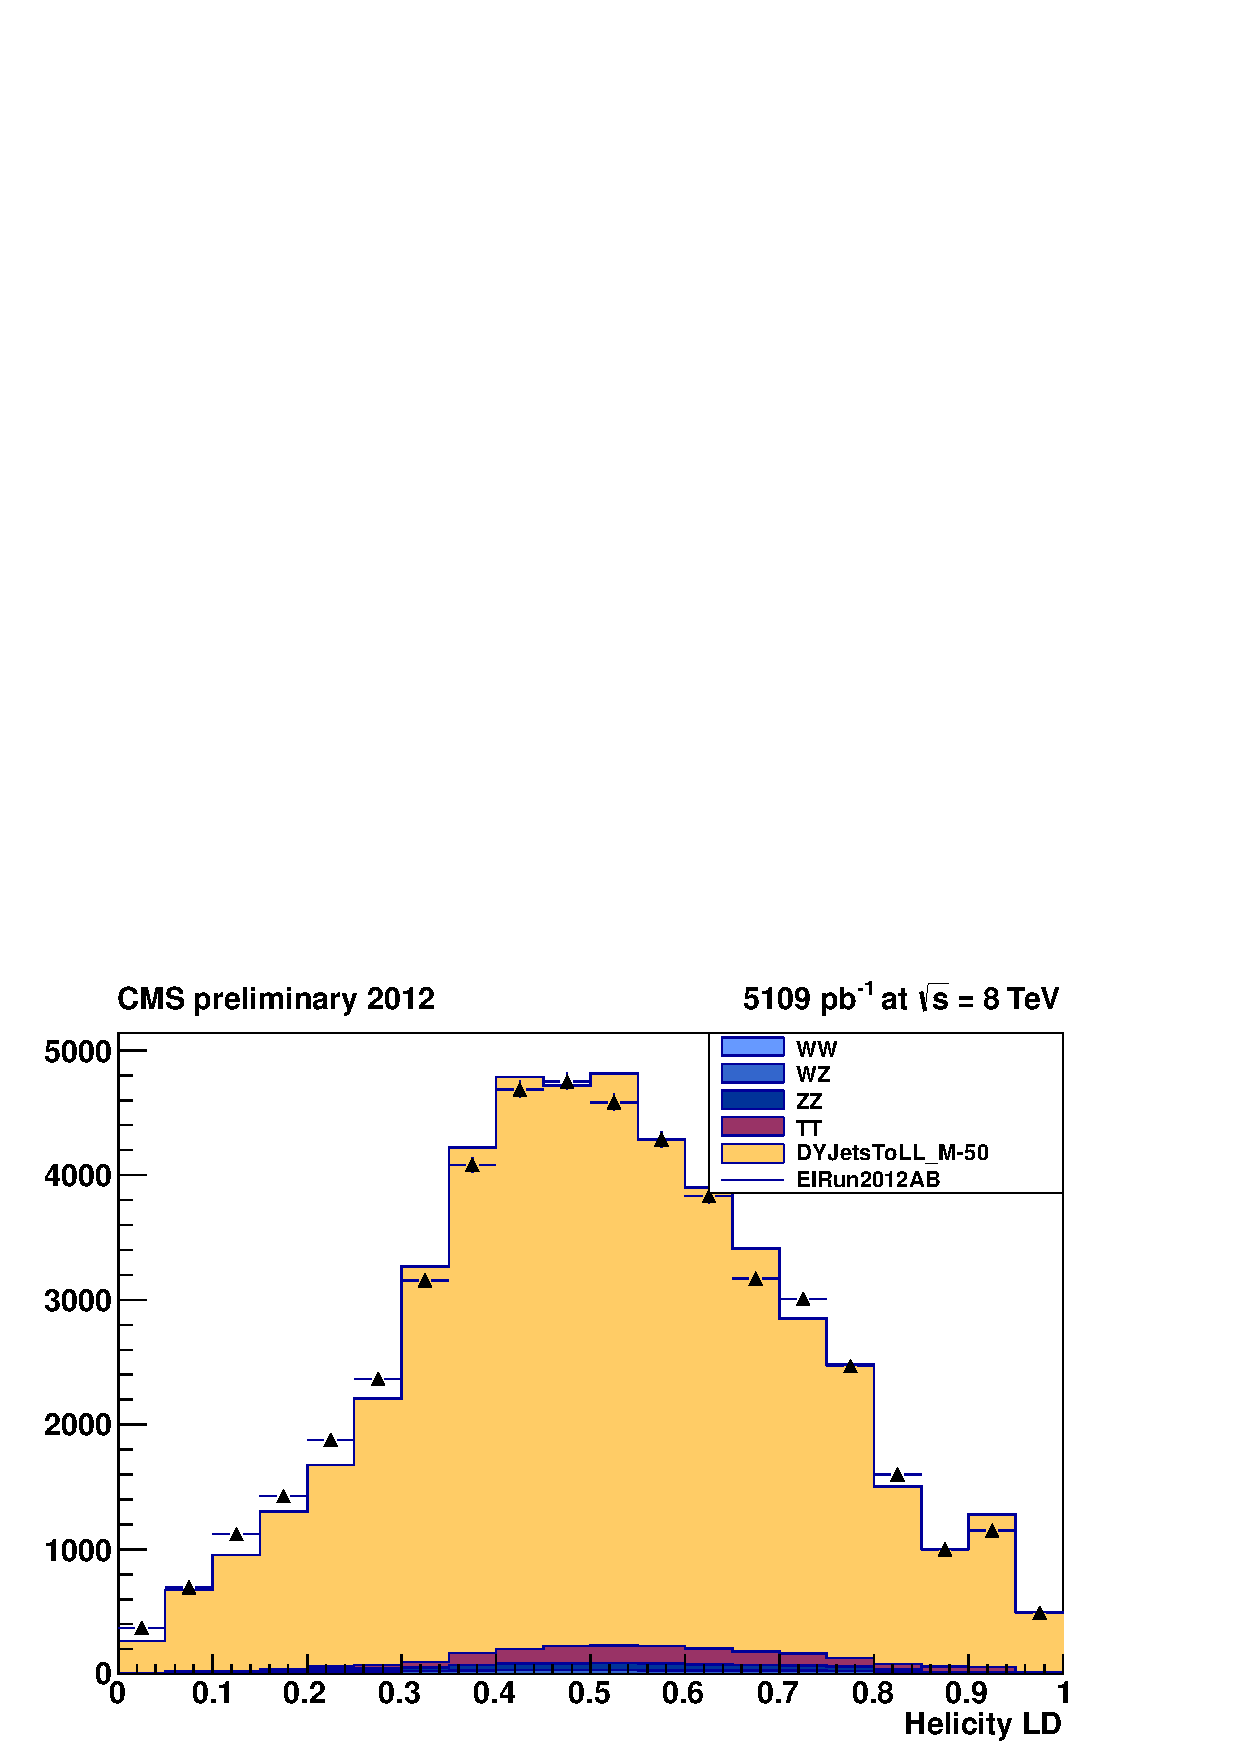
\includegraphics[width=0.33\textwidth]{images/plots/HelyLDRefit_ElRun2012.png}
\end{center}
\end{frame}


\begin{frame}{Muon Helicity and Production Angles}
\begin{center}
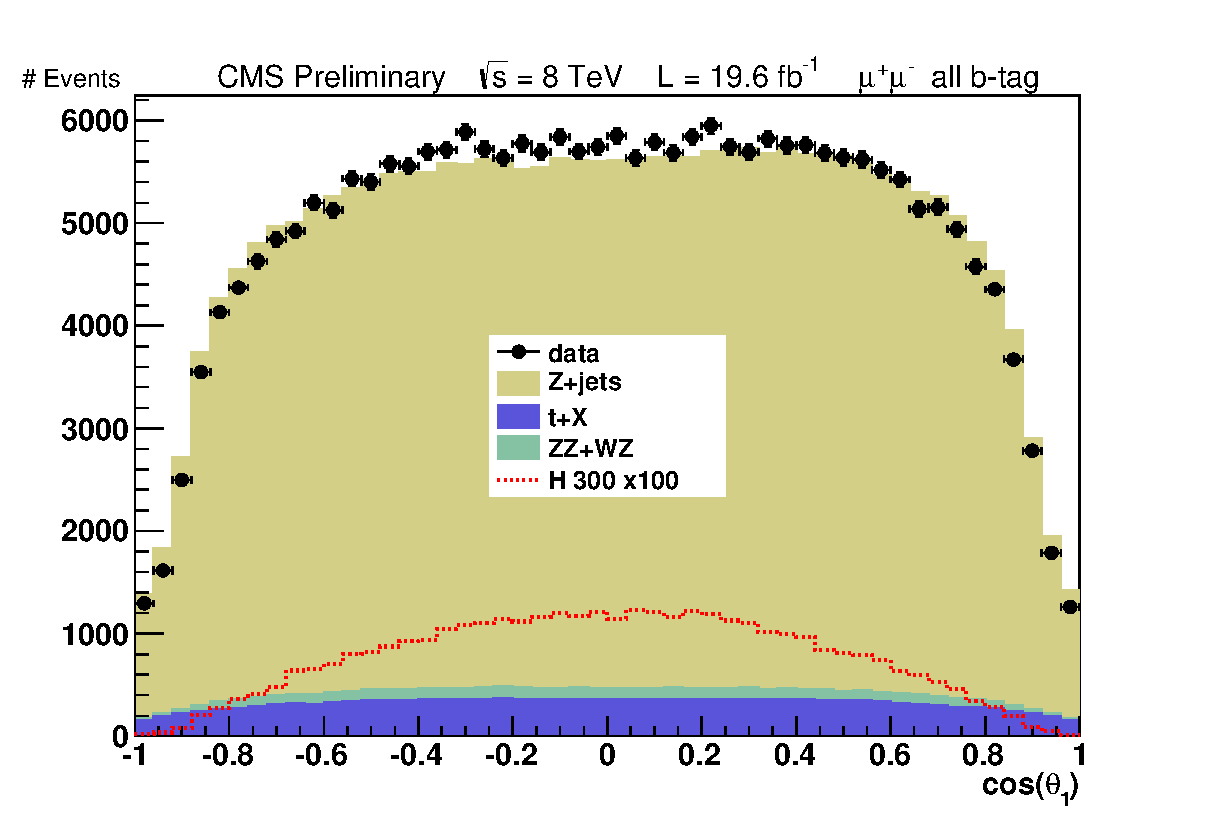
\includegraphics[width=0.33\textwidth]{images/preselection/mu/costheta1.eps}
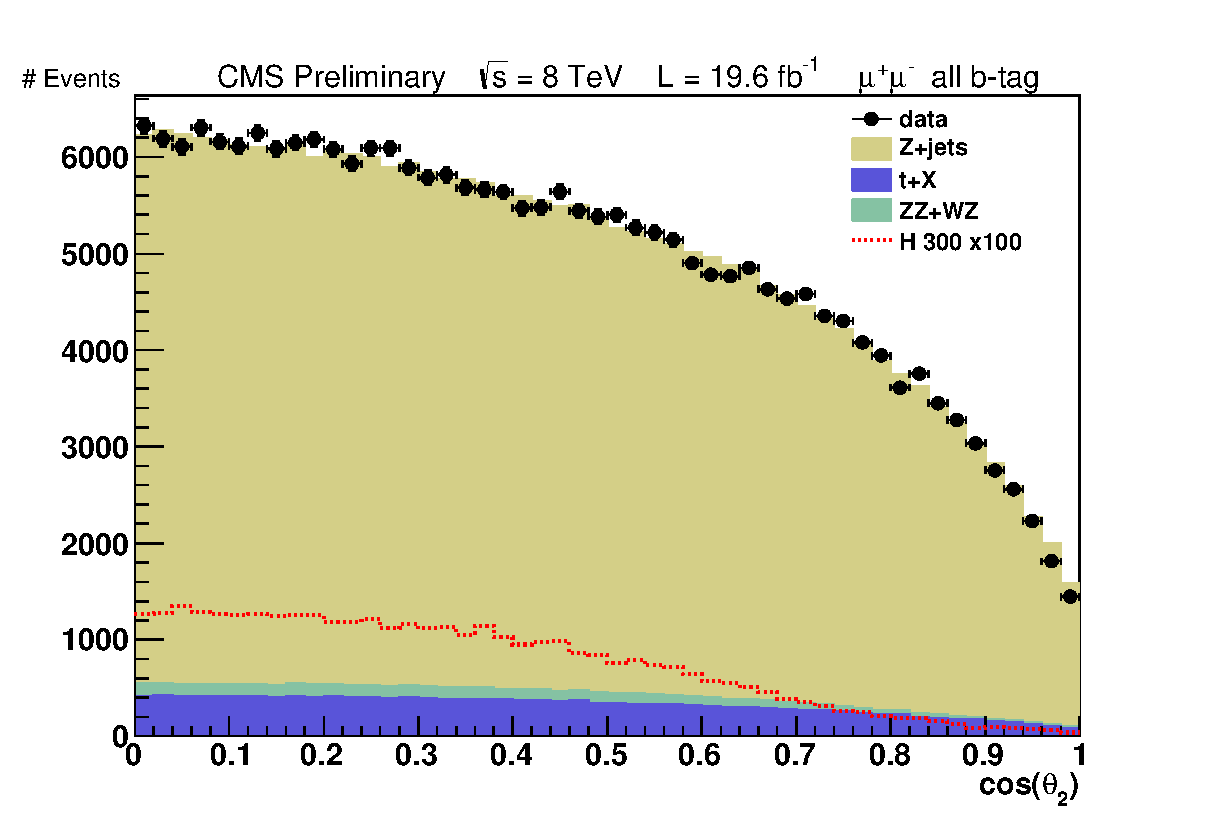
\includegraphics[width=0.33\textwidth]{images/preselection/mu/costheta2.eps}
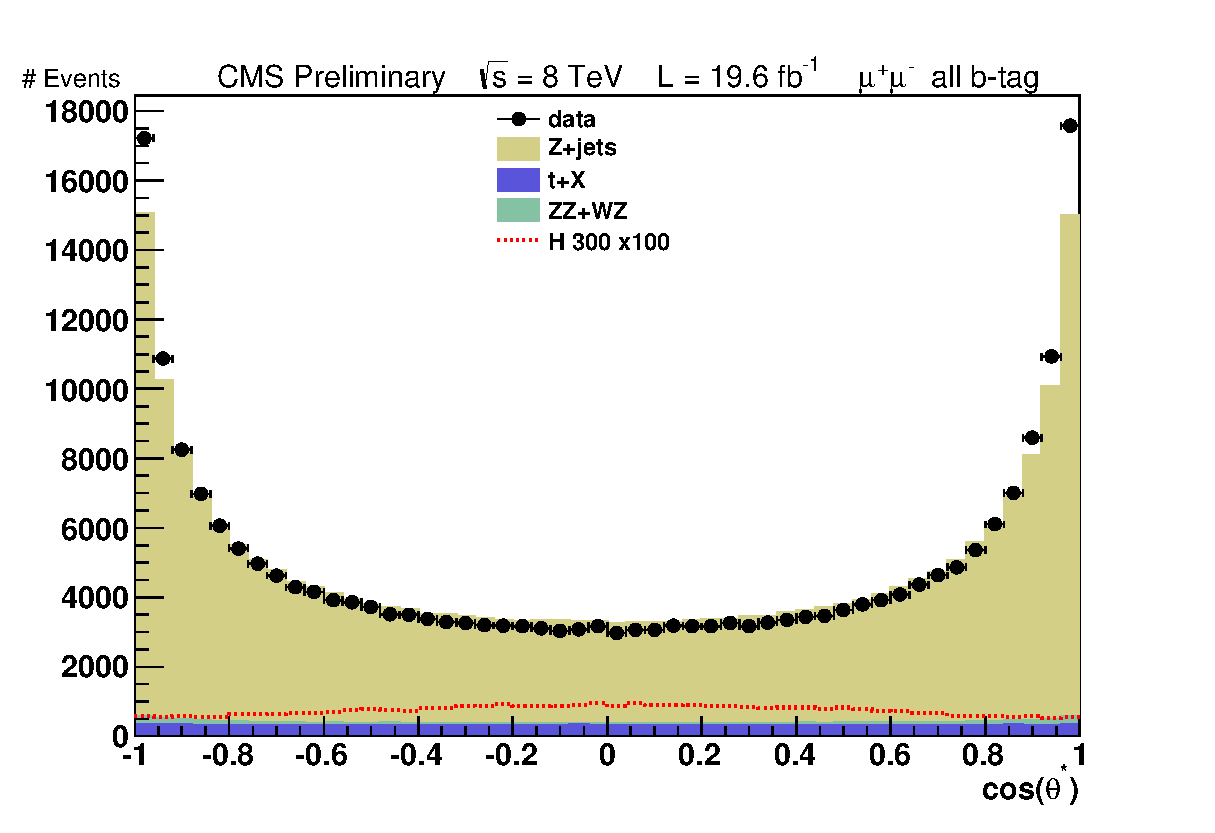
\includegraphics[width=0.33\textwidth]{images/preselection/mu/costhetast.eps}
\\
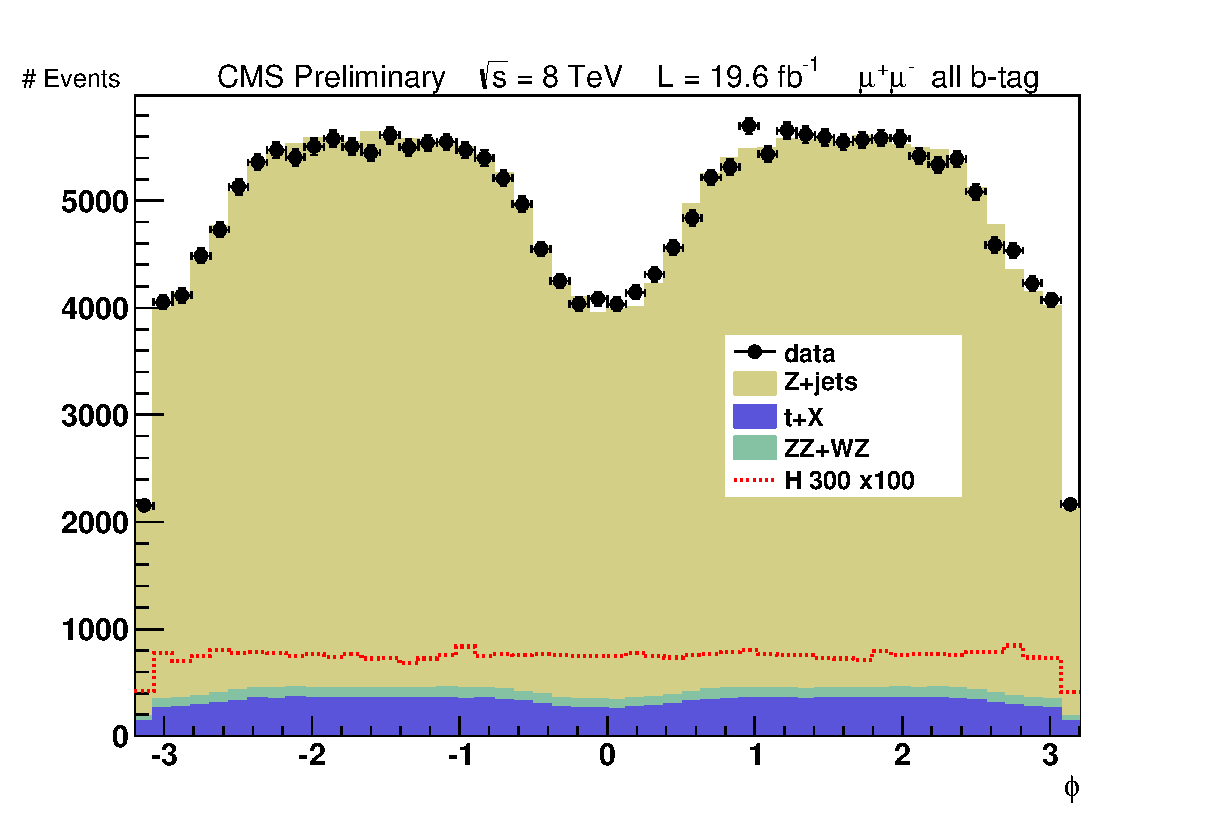
\includegraphics[width=0.33\textwidth]{images/preselection/mu/phi.eps}
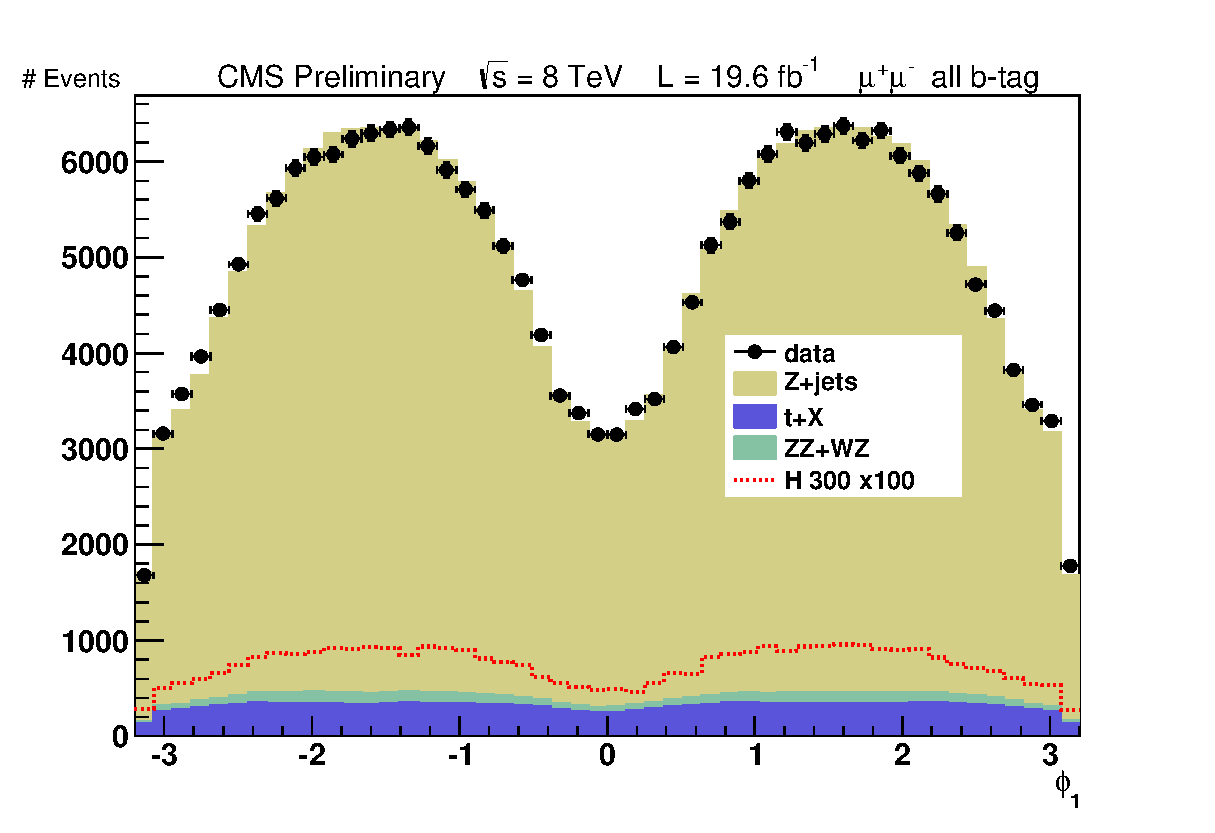
\includegraphics[width=0.33\textwidth]{images/preselection/mu/phi1.eps}

\end{center}
\end{frame}



\begin{frame}{Signal Angular Distribution Fits}
\begin{center}
Example fits at for 500 GeV (475 - 550 GeV).
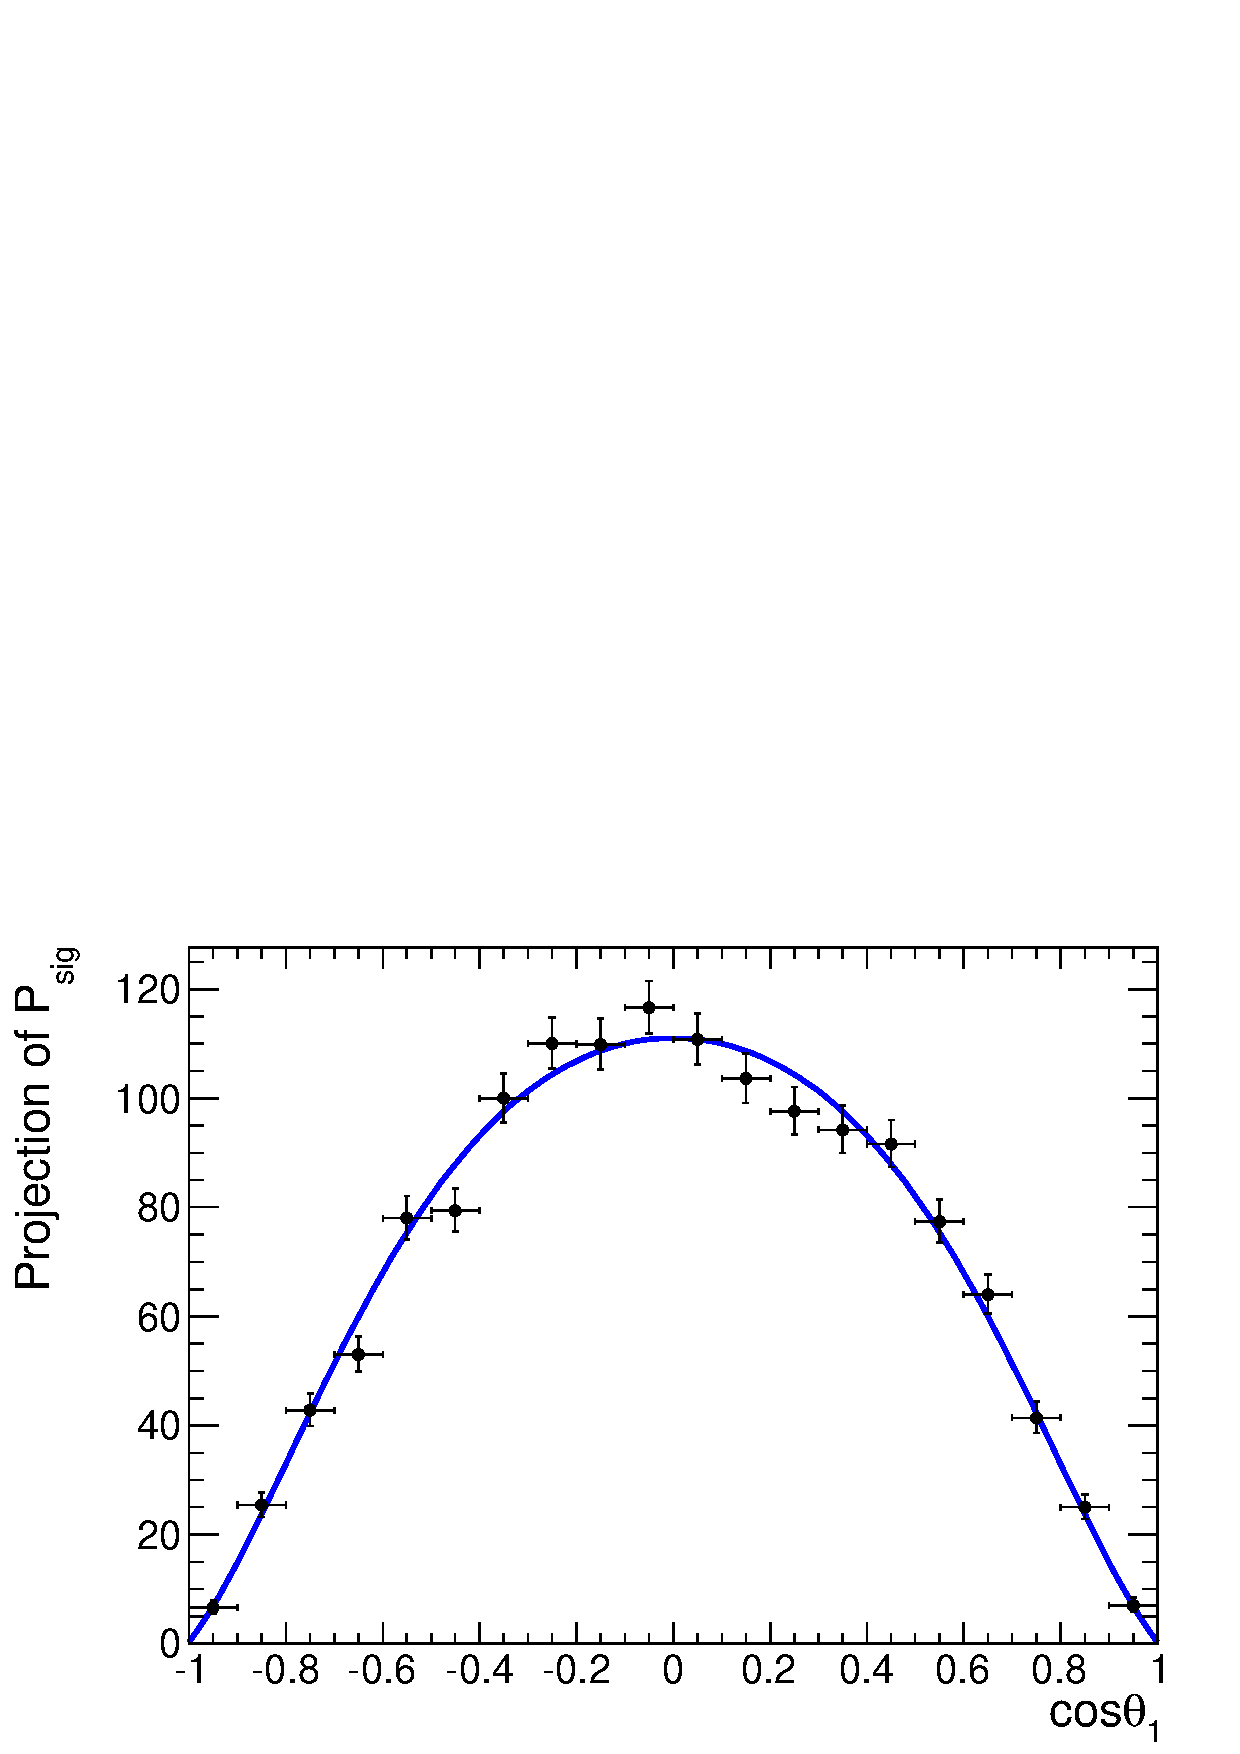
\includegraphics[width=0.33\textwidth]{images/plots/sigPDF_CosTheta1proj_500.pdf}
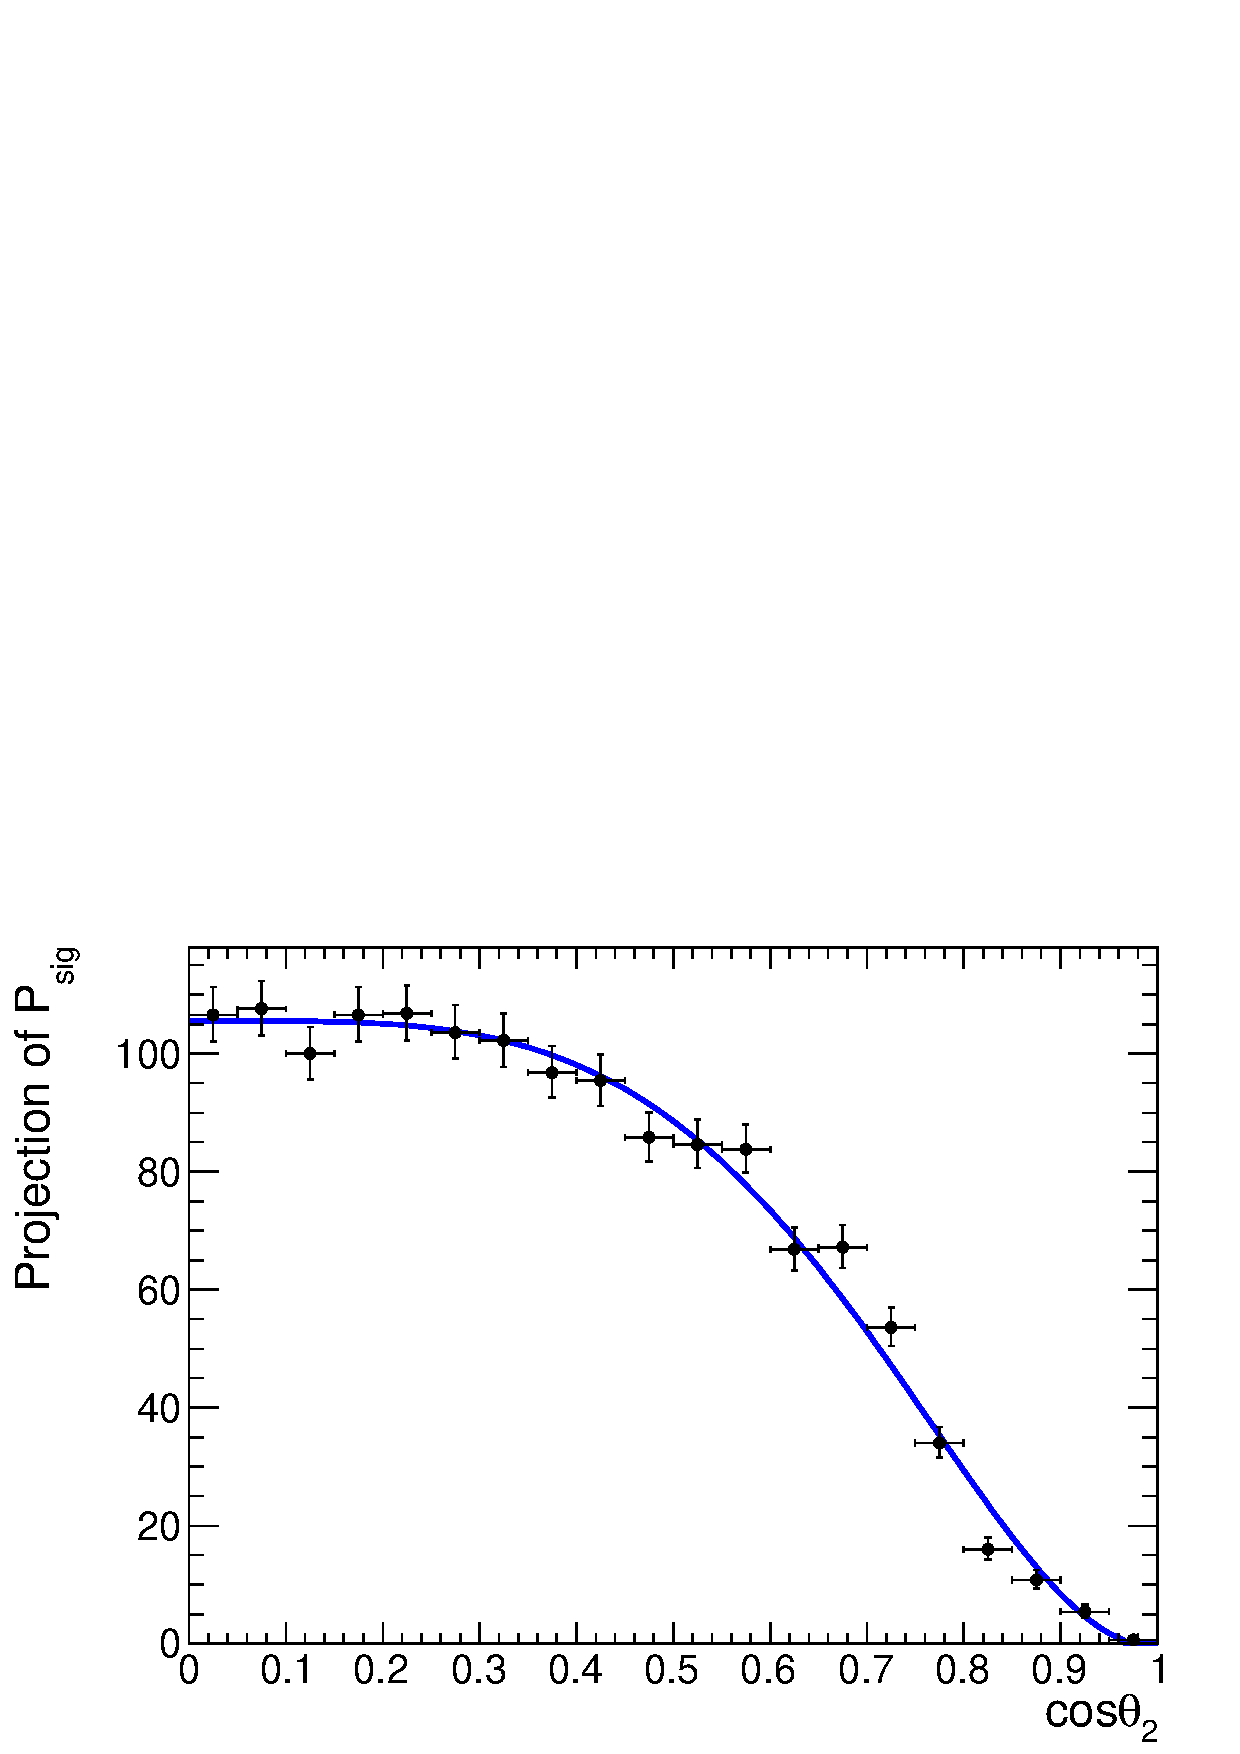
\includegraphics[width=0.33\textwidth]{images/plots/sigPDF_CosTheta2proj_500.pdf}
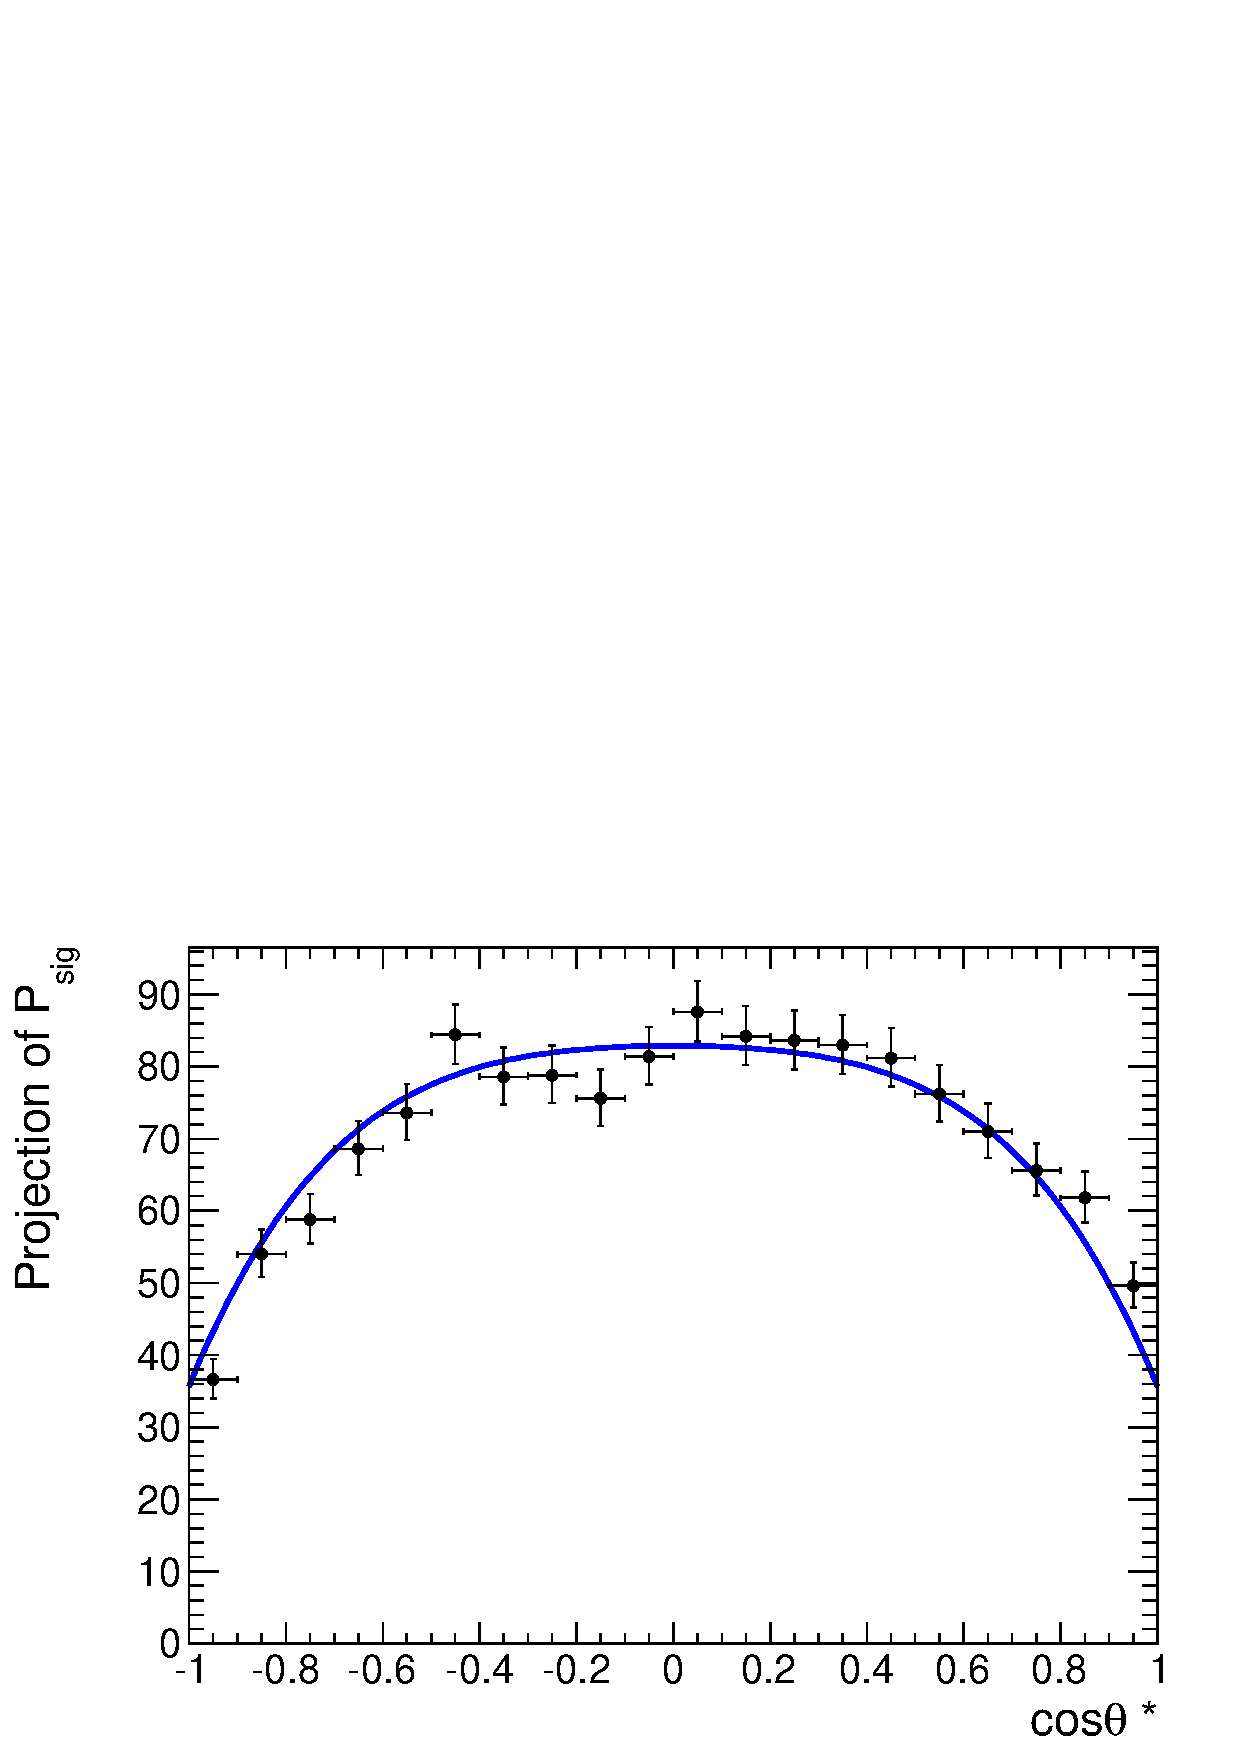
\includegraphics[width=0.33\textwidth]{images/plots/sigPDF_CosThetaSproj_500.pdf}
\\
\includegraphics[width=0.33\textwidth]{images/plots/sigPDF_Phiproj_500.pdf}
\includegraphics[width=0.33\textwidth]{images/plots/sigPDF_PhiStar1proj_500.pdf}

%sigPDF_CosTheta1proj_500.pdf  sigPDF_CosTheta2proj_500.pdf  sigPDF_CosThetaSproj_500.pdf  sigPDF_Phiproj_500.pdf  sigPDF_PhiStar1proj_500.pdf

\end{center}
\end{frame}

\begin{frame}{Helicity LD Distribution and Cuts}
\begin{center}
$LD = \dfrac{P_{sig}}{P_{sig} + P_{bkg}}$
\\
%\vpace{1em}
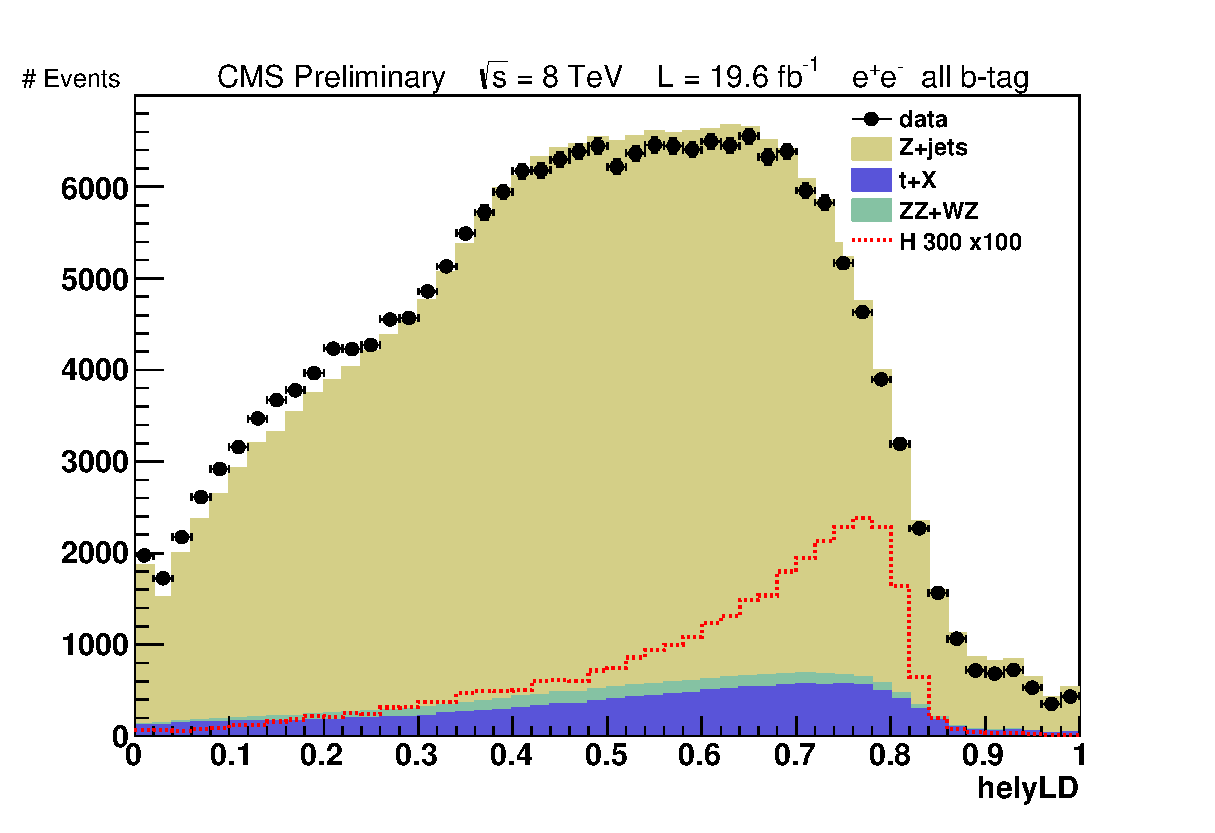
\includegraphics[width=0.5\textwidth]{images/preselection/el/helyLD.eps}
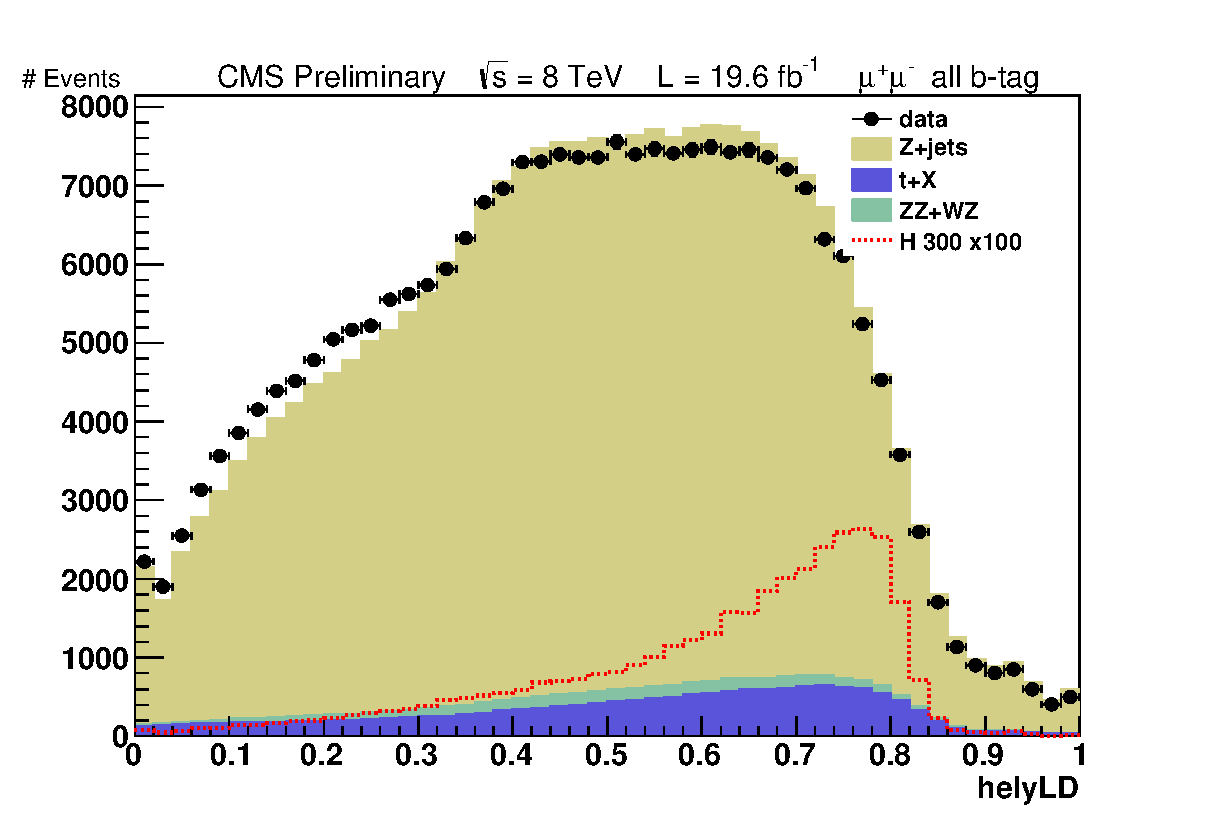
\includegraphics[width=0.5\textwidth]{images/preselection/mu/helyLD.eps}\\
\vspace{2em}
\tiny
An explanation of the shape discrepancy is given in the backup slides.
\end{center}
\end{frame}

\begin{frame}{HelyLD Optimization}
%\begin{center}

  \begin{columns}
    \begin{column}{0.3\textwidth}
      %\begin{center}
        We do an optimization for the cut on the HelyLD maximizing the Punzi equation:\\ 
        \vspace{1em}
        $\dfrac{\dfrac{\#\ signal}{\#\ total\ signal}}{0.98 + \sqrt{B}}$
      %\end{center}
    \end{column}
    \begin{column}{0.7\textwidth}
      %\includegraphics[width=0.99\linewidth]{images/two_300.eps}
      \includegraphics[width=0.99\linewidth]{images/hely_optimization.eps}
    \end{column}
  \end{columns}
\begin{center}
We cut on 0.5 which is within 5\% of the optimal value for all Higgs mass values, b-tag regions, and lepton types.
\end{center}
\end{frame}








\begin{frame}{Missing Transverse Energy}
\footnotesize
Our signal should not have any Missing Transverse Energy ($E_T^{miss}$, MET) from neutrinos.
MET significance is a measure of how likely the MET we see is real(not from detector effects).\\
\begin{block}{}
\begin{center}
$MET\ Significance = 2ln\lambda(MET) = 2ln \dfrac{L(MET_{true} = MET_{measured})}{L(MET_{true} = 0)}$
\end{center}
\end{block}

This is particularly useful to suppress the $\Pqt \Paqt$ background in the 2-tag region (b-tagging on next slide), but we apply a cut on MET significance > 10 to all categories.  
\\
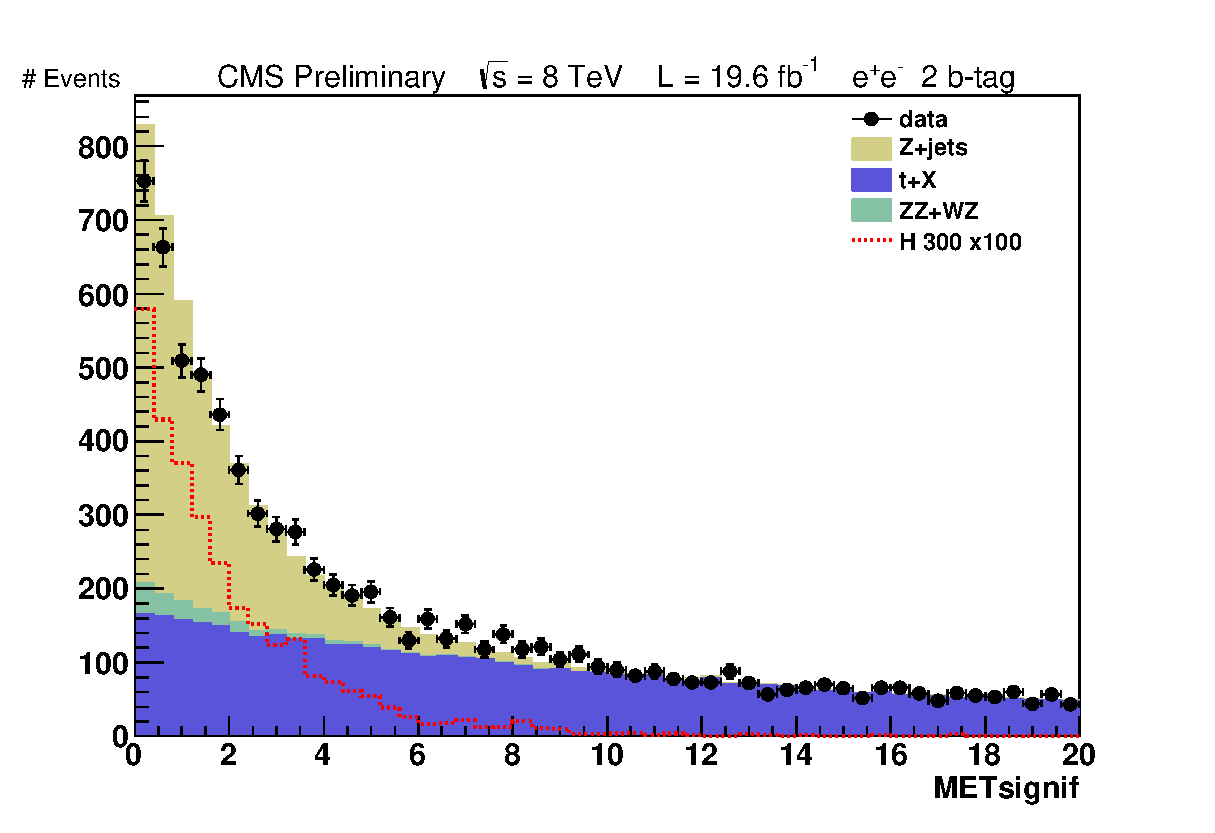
\includegraphics[width=0.5\linewidth]{images/preselection/2/el/METsignif.eps}
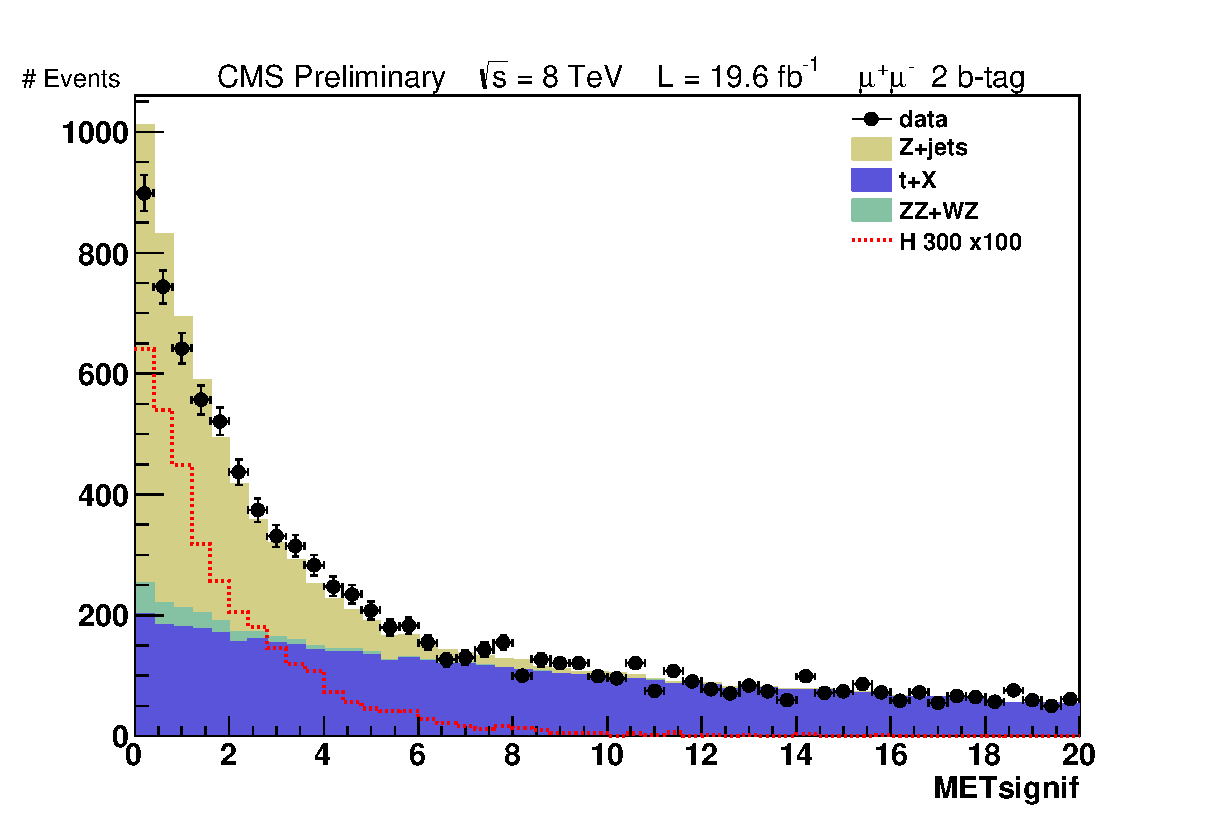
\includegraphics[width=0.5\linewidth]{images/preselection/2/mu/METsignif.eps}
\end{frame}

















\begin{frame}{$b$-tagging}
  \begin{columns}
    \begin{column}{0.4\textwidth}
      \begin{itemize}
        {\small
        \item Using {\bf JP algorithm}
          
        \item
          We are looking for heavy quarks (b,c)
        \item
          There are ``loose''(0.275) and ``medium''(0.545) working points that are defined by the b-tag group that we use to classify our events.
        }
      \end{itemize}
      
    \end{column}
    
    \begin{column}{0.6\textwidth}
      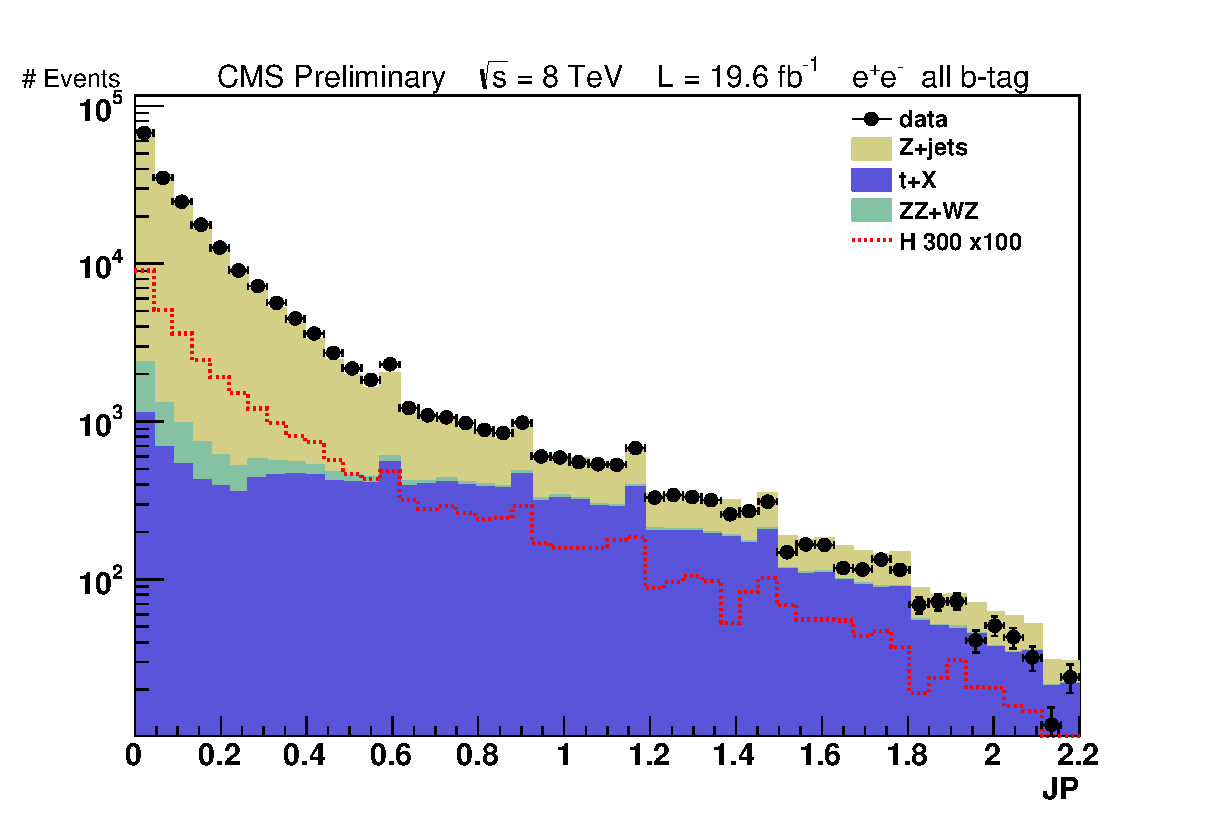
\includegraphics[width=0.99\textwidth]{images/preselection/el/j0jp_log.eps}
%images/JPJet_MuRun2012_LOG.eps}
    \end{column}
  \end{columns}
 \begin{center}
  \begin{tabular}{|c|c|}\hline
    0 - tag  & Both Jets < Loose \\ \hline 
    1 - tag  & > Loose and < Medium \\ \hline
    2 - tag  & > Loose and > Medium \\ \hline
  \end{tabular}
  \end{center}
\end{frame}


\begin{frame}{Best Higgs Candidate}
\footnotesize
When there are multiple candidates in the same event we apply a string of logic to select which is the candidate that we are going to keep.\\
\vspace{1em}
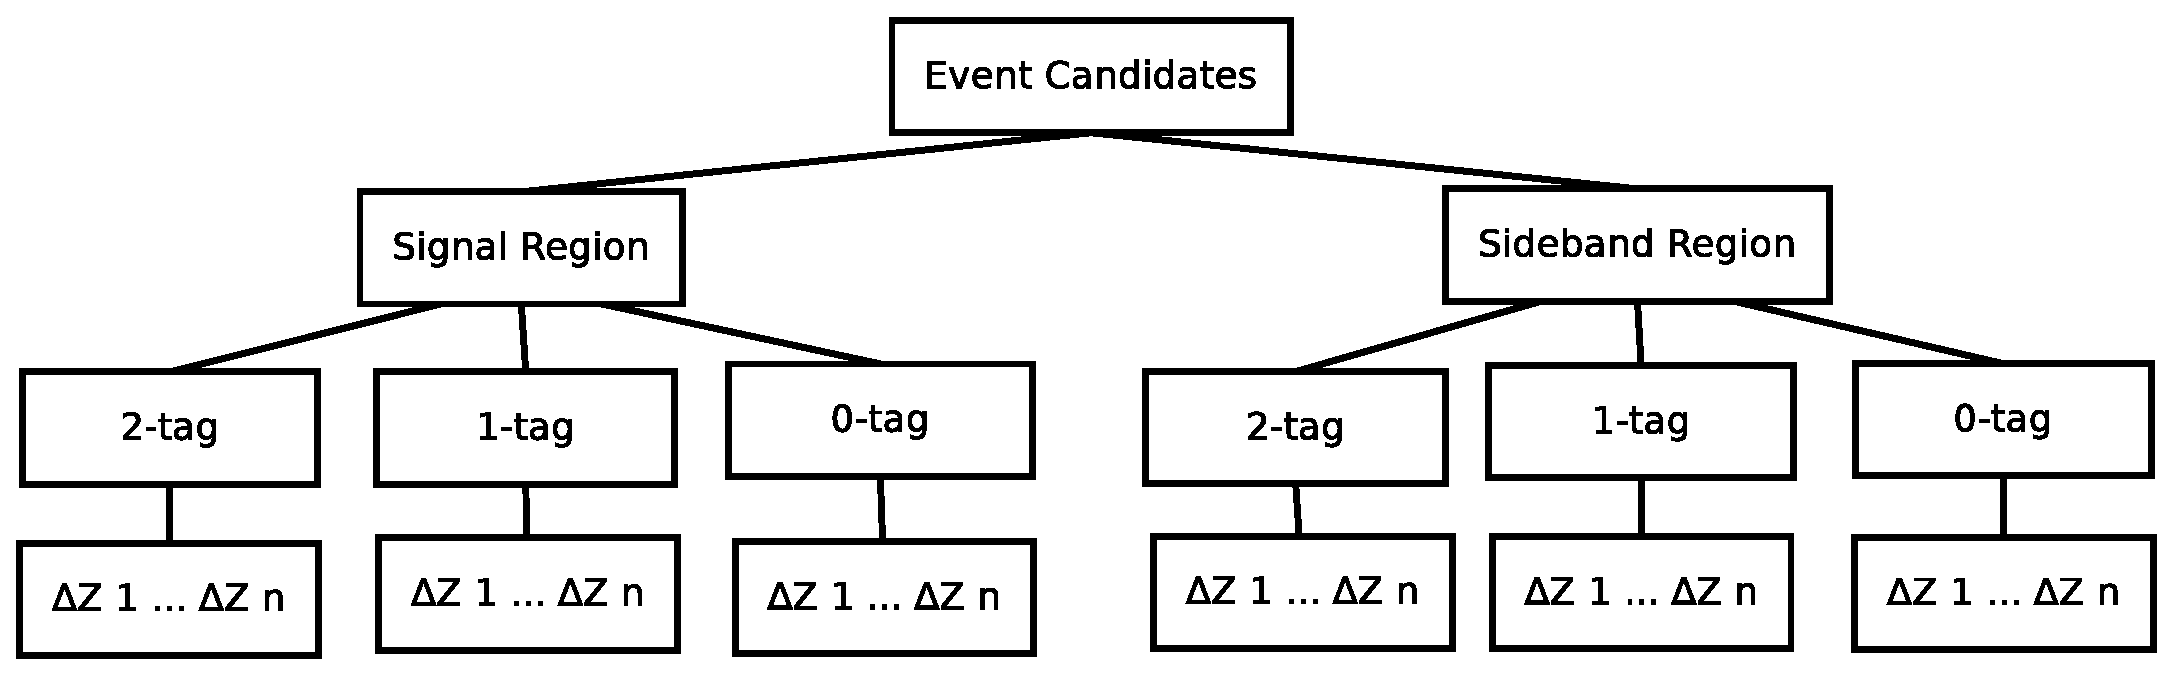
\includegraphics[width=0.99\textwidth]{images/final_cand.eps}\\
\vspace{1em}
\begin{center}
$\Delta Z = |M_{\Plp \Plm} - m_Z| + |M_{JJ} - m_Z|$\\
$m_Z$ is the nominal mass of the Z boson\\
$\Delta Z 1 ...$ $Z n$ is the candidates sorted by $\Delta Z$ smallest to largest.\\
\end{center}
\vspace{1em}
When all candidates are sorted we keep the candidate that is furthest to the left.
\end{frame}






\begin{frame}{Final Region m$_{ZZ}$ Plots}
\begin{center}
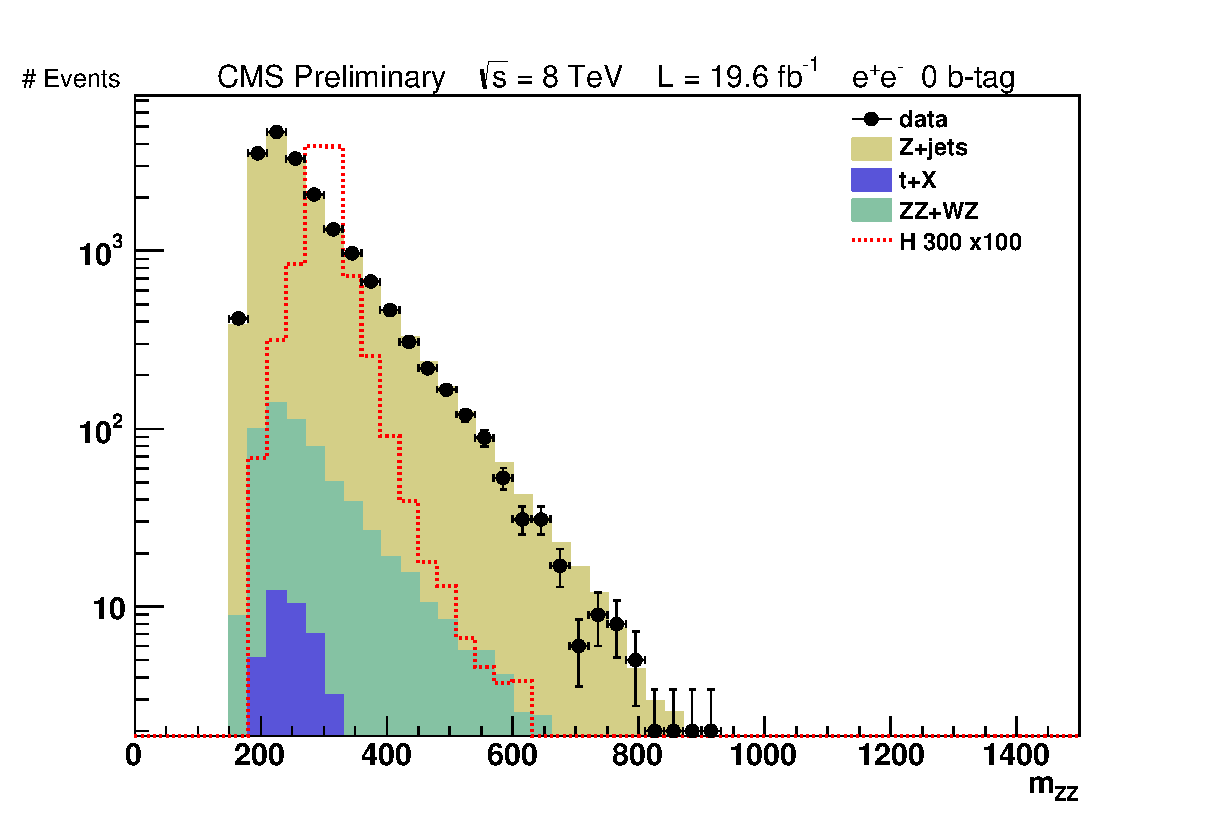
\includegraphics[width=0.33\textwidth]{images/final/0/el/mZZ_signal_log.eps}
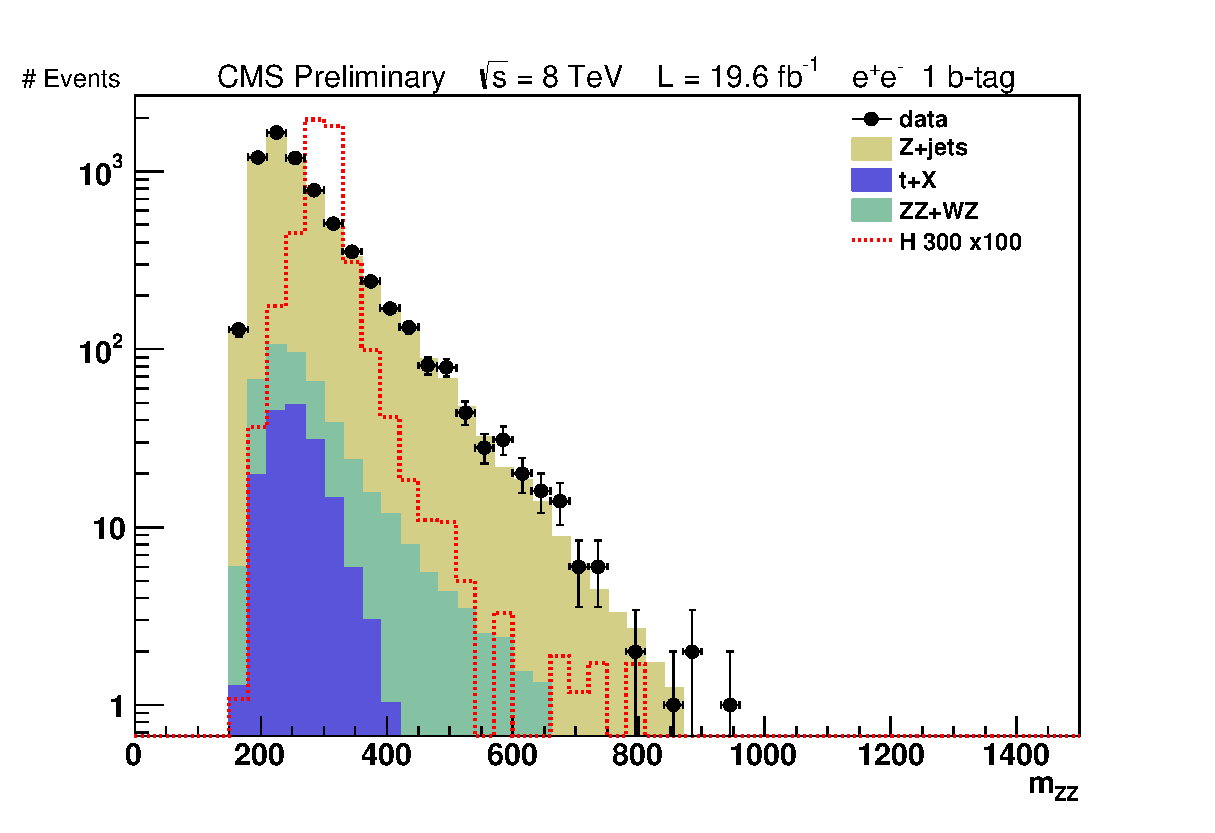
\includegraphics[width=0.33\textwidth]{images/final/1/el/mZZ_signal_log.eps}
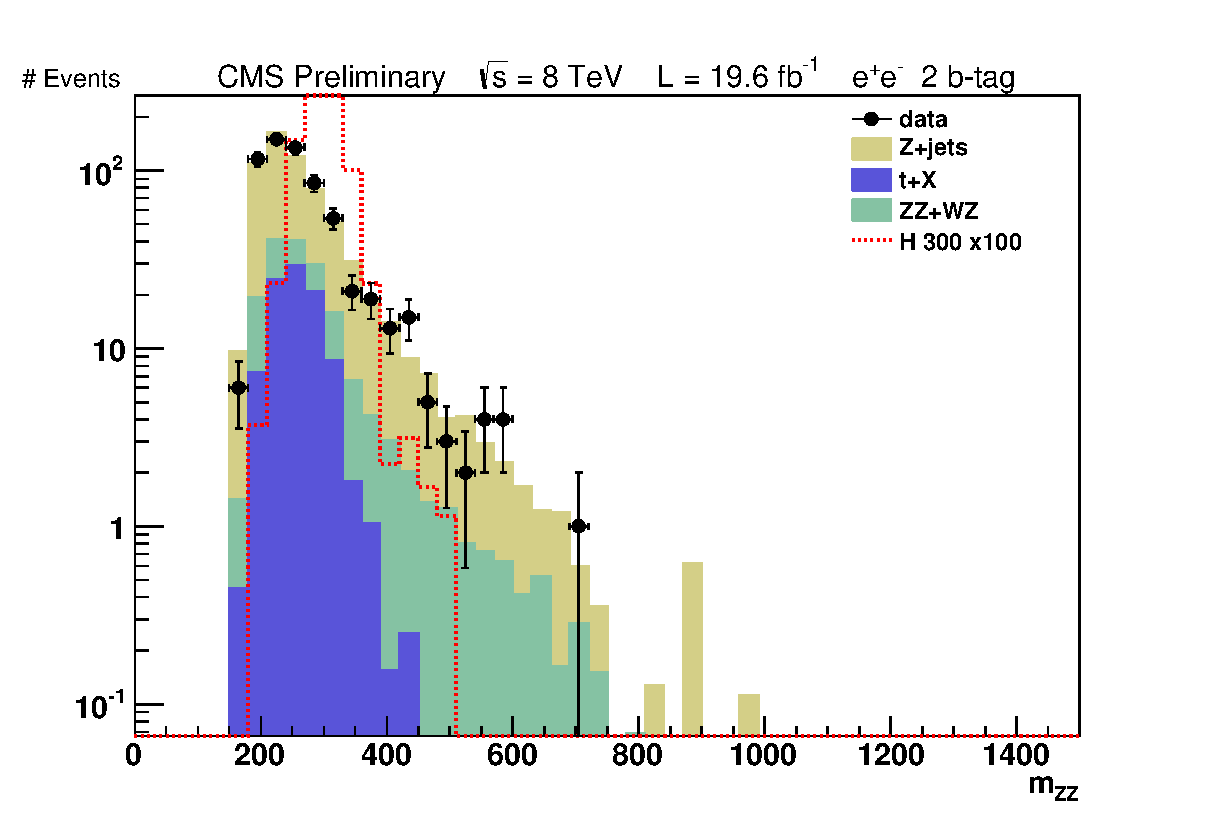
\includegraphics[width=0.33\textwidth]{images/final/2/el/mZZ_signal_log.eps}\\
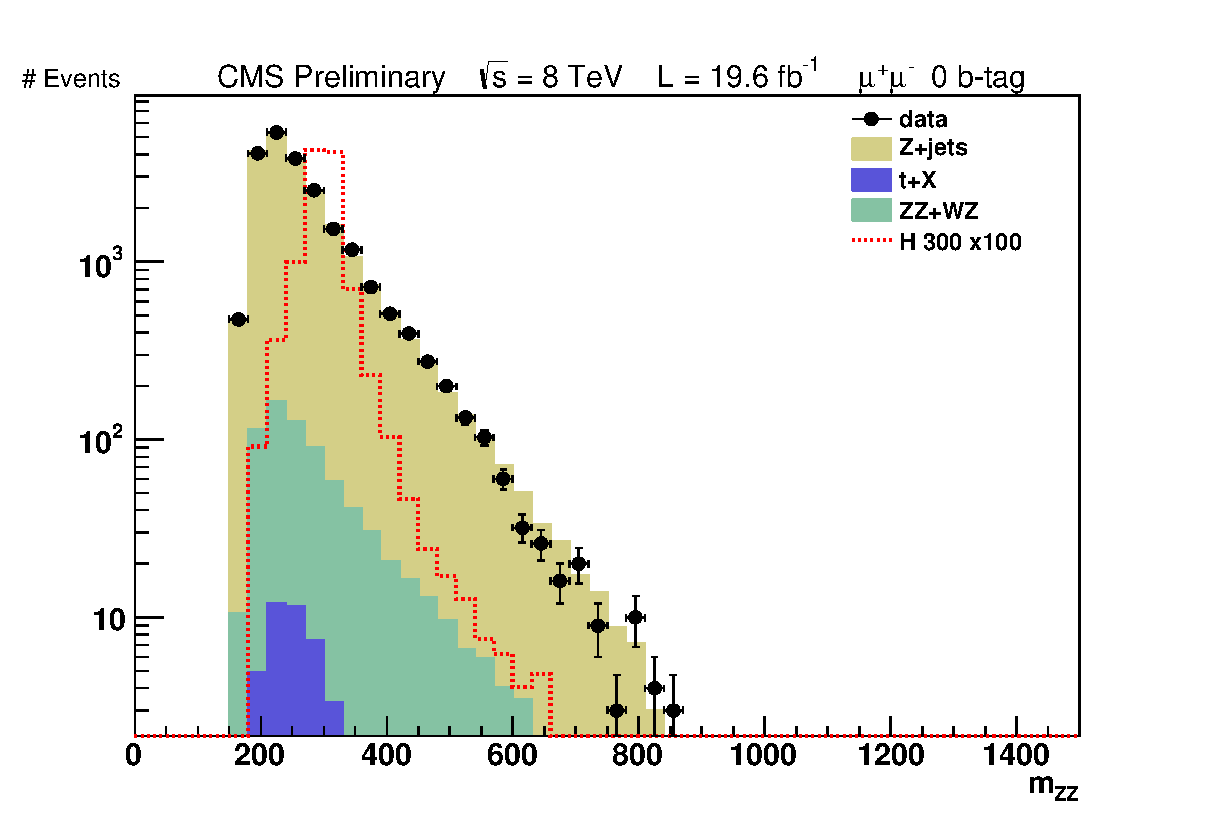
\includegraphics[width=0.33\textwidth]{images/final/0/mu/mZZ_signal_log.eps}
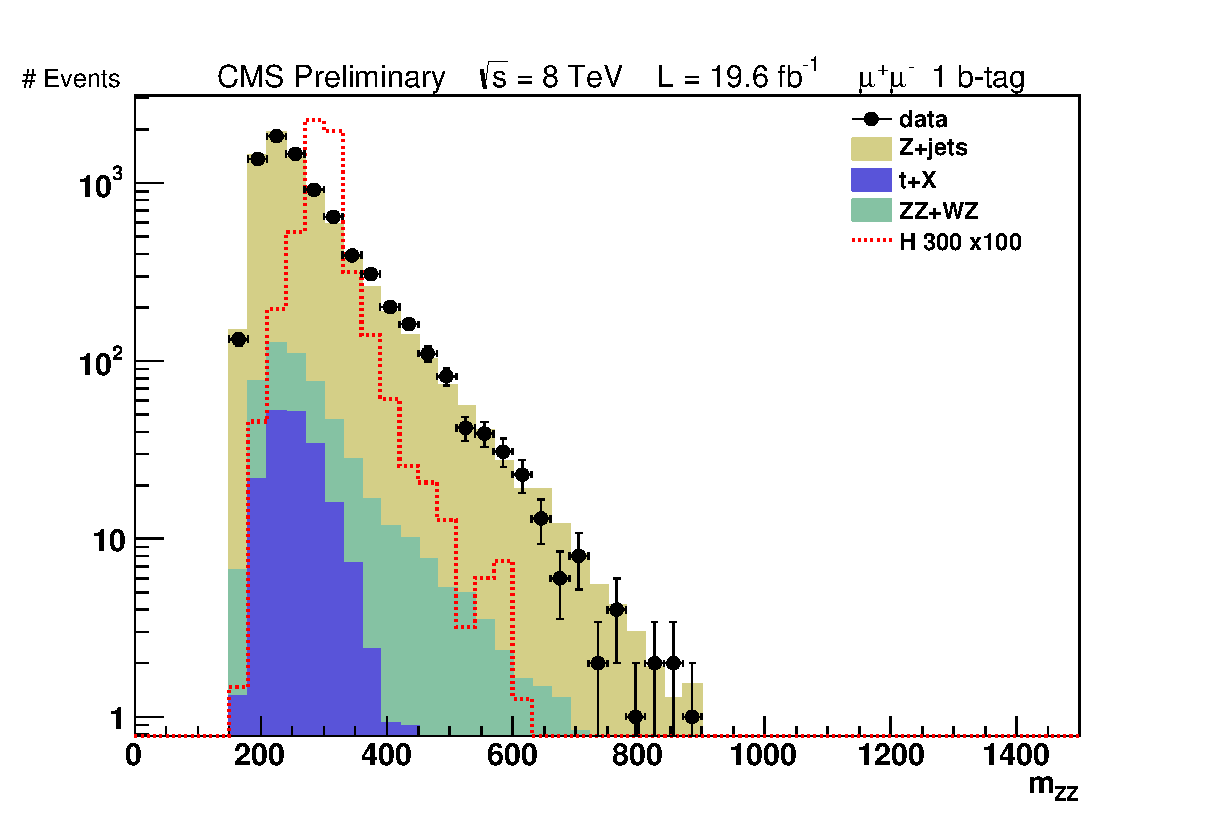
\includegraphics[width=0.33\textwidth]{images/final/1/mu/mZZ_signal_log.eps}
\includegraphics[width=0.33\textwidth]{images/final/2/mu/mZZ_signal_log.eps}
\end{center}
\end{frame}


%%%%%%%%%%%%%%%%%%%%%%%%%%%%%%%%%%%%%%%%%%%%%%%%%%%%%%%%%%%%%%%%%%%%%%%%%%%%%%%%%%%%%%%%%


%\begin{frame}{Window Cuts}
%\begin{center}
%Previous values of the windows around the $m_{LL}$ and $m_{JJ}$ peaks were done by eye. We optimized these windows to maximize $\dfrac{S}{\sqrt{S+B}}$ for a %wide range of Higgs masses.
%\includegraphics[width=0.33\textwidth]{images/zjj_s_sb_zero.eps}
%\includegraphics[width=0.33\textwidth]{images/zjj_s_sb_one.eps}
%\includegraphics[width=0.33\textwidth]{images/zjj_s_sb_two.eps}
%\end{center}
%\end{frame}

%\begin{frame}{Signal and Sideband Regions}
%  {\bf Study Regions}
%  \begin{itemize}
%  \item 
%   Signal Region is 76 < m$_{ll}$ < 106 GeV and 71 < m$_{jj}$ < 111 GeV
%  \item 
%    Also we are looking at the sidebands region, defined as 60< m$_{jj}$ <71 GeV || 111< m$_{jj}$ <130 GeV (i.e. outside signal window 75< mjj < 105 GeV).
%  \end{itemize}
 % \includegraphics[width=0.5\textwidth]{images/zjjmass_ElRun2012.eps}
 % \includegraphics[width=0.5\textwidth]{images/zjjmass_MuRun2012.eps}
%  \begin{center}
%    \includegraphics[width=0.6\textwidth]{images/mJJ_signal_sideband.eps}
%  \end{center}

 % \begin{columns}
 %   \begin{column}{0.4\textwidth}
 %      \begin{block}{}
 %       \begin{center}
 %         All plots are either inclusive pre-selection or are in the sidebands.\\
 %        \end{center}
 %     \end{block}
 %   \end{column}
 %    \begin{column}{0.6\textwidth}
 %     \includegraphics[width=0.9\textwidth]{images/zjjmass_MuRun2012_blind.eps}
 %    \end{column}
 % \end{columns}
 
%\end{frame}

%\begin{frame}{Data-MC plots Pretag}
%  \begin{center}
%    Electrons\\
%    $\phi$ \hspace{7.5em} $\phi^{*}$ \hspace{7.5em} Helicity LD
%    \\
%  \includegraphics[width=0.33\textwidth]{images/phiRefit_ElRun2012.eps}
%  \includegraphics[width=0.33\textwidth]{images/phiStarRefit_ElRun2012.eps}
%  \includegraphics[width=0.33\textwidth]{images/HelyLDRefit_ElRun2012.eps}\\
%  $cos\theta_{1}$ \hspace{7.5em} $cos\theta_{1}^{*}$ \hspace{7.5em} $cos\theta_{2}$
%  \includegraphics[width=0.33\textwidth]{images/cosTheta1Refit_ElRun2012.eps}
%  \includegraphics[width=0.33\textwidth]{images/cosTheta1StarRefit_ElRun2012.eps}
%  \includegraphics[width=0.33\textwidth]{images/cosTheta2Refit_ElRun2012.eps}
%  \end{center}
%\end{frame}



%\begin{frame}{Data-MC plots Pretag}
%  \begin{center}
%    Muons\\
%    $\phi$ \hspace{7.5em} $\phi^{*}$ \hspace{7.5em} Helicity LD
%    \\
%  \includegraphics[width=0.33\textwidth]{images/phiRefit_MuRun2012.eps}
%  \includegraphics[width=0.33\textwidth]{images/phiStarRefit_MuRun2012.eps}
%  \includegraphics[width=0.33\textwidth]{images/HelyLDRefit_MuRun2012.eps}\\
%  $cos\theta_{1}$ \hspace{7.5em} $cos\theta_{1}^{*}$ \hspace{7.5em} $cos\theta_{2}$
%  \includegraphics[width=0.33\textwidth]{images/cosTheta1Refit_MuRun2012.eps}
%  \includegraphics[width=0.33\textwidth]{images/cosTheta1StarRefit_MuRun2012.eps}
%  \includegraphics[width=0.33\textwidth]{images/cosTheta2Refit_MuRun2012.eps}
%  \end{center}
%\end{frame}

